% last edited 2008-11-22

\chapter{Rules for differentiating standard elementary forms}

 
%33. 
\section{Importance of General Rule}
\label{sec:33}

The General Rule for differentiation, given in the 
last chapter, %p. 29 [§ 31], 
\S \ref{sec:31},
is fundamental, being found directly from the definition 
of a derivative. %% new grammatical change
It is very important that the 
student should be thoroughly familiar with it. However, the 
process of applying the rule to examples in general has been 
found too tedious or difficult; consequently special rules 
have been derived from the General Rule for differentiating 
certain standard forms of frequent occurrence in order to facilitate 
the work.

It has been found convenient to express these special rules by 
means of formulas, a list of which follows. The student 
should not only memorize each formula when deduced, but 
should be able to state the corresponding rule in words. In 
these formulas $u$, $v$, and $w$ denote variable quantities 
which are functions of $x$, and are differentiable.

\begin{center}
Formulas for differentiation
\end{center}

\begin{tabular}{lc}
I 	&  	$\frac{dc}{dx} 	= 0$\\
 & \\
II &	  	$\frac{dx}{dx} 	= 1$\\
 & \\
III &	  	$\frac{d}{dx}(u + v - w) 	= \frac{du}{dx}\ +\ \frac{dv}{dx}\ -\ \frac{dw}{dx}$\\
 & \\
IV 	 & 	$\frac{d}{dx} (cv) 	= c \frac{dv}{dx}$\\
 & \\
V 	 & 	$\frac{d}{dx} (uv) 	= u\frac{dv}{dx}\ +\ v\frac{du}{dx}$\\
 & \\
\end{tabular}

\newpage
\begin{center}
Formulas for differentiation (cont.)
\end{center}

The function $\vers$ used in (XVII) below is defined by $\vers\ v=1-\cos\ v$. 
See \url{http://en.wikipedia.org/wiki/Versine} for a history of the versine
function.

\vskip .4in

\begin{tabular}{lc}
VI &	  $	\frac{d}{dx} \left ( v^n \right ) = nv^{n-1} \frac{dv}{dx}$\\
 & \\
VI 	a &$	\frac{d}{dx} \left ( x^n \right ) = nx^{n - 1}$\\
 & \\
VII 	&  $	\frac{d}{dx} \left ( \frac{u}{v} \right ) = \frac{v\frac{du}{dx}\ -\ u\frac{dv}{dx}}{v^2}$\\
 & \\
VII 	a &	$\frac{d}{dx} \left ( \frac{u}{c} \right ) = \frac{\frac{du}{dx}}{c}$\\
 & \\
VIII 	 & 	$\frac{d}{dx} \left ( \log_a v \right ) = \log_a\ e\ \cdot\ \frac{\frac{dv}{dx}}{v}$\\
 & \\
IX &	$  	\frac{d}{dx} \left ( a^v \right ) = a^v\ \log\ a\ \frac{dv}{dx}$\\
 & \\
IX 	a &	$\frac{d}{dx} \left ( e^v \right ) = e^v \frac{dv}{dx}$\\
 & \\
X &	  	$\frac{d}{dx} \left ( u^v \right ) = vu^{v-1} \frac{du}{dx}\ +\ \log\ u\ \cdot\ u^v \frac{dv}{dx}$\\
 & \\
XI  &	  	$\frac{d}{dx} (\sin\ v) = \cos\ v \frac{dv}{dx}$\\
 & \\
XII  &	 $ 	\frac{d}{dx}(\cos\ v) = -\sin\ v \frac{dv}{dx}$\\
 & \\
XIII  &	 $ 	\frac{d}{dx}(\tan\ v) =	\sec^2 v \frac{dv}{dx}$\\
 & \\
XIV  &	 $ 	\frac{d}{dx}(\cot\ x) 	= -\csc^2 v \frac{dv}{dx}$\\
 & \\
XV  &	  $	\frac{d}{dx}(\sec\ v) 	= \sec\ v\ \tan\ v \frac{dv}{dx}$\\
 & \\
XVI  &	 $ 	\frac{d}{dx} (\csc\ v) 	= -\csc\ v\ \cot\ v \frac{dv}{dx}$\\
 & \\
XVII  &	 $ 	\frac{d}{dx} (\vers\ v) = \sin\ v \frac{dv}{dx}$\\
 & \\
XVIII  &	 $\frac{d}{dx} (\arcsin\ v) = \frac{\frac{dv}{dx}}{\sqrt{1 - v^2}}$\\
 & \\
XIX  &	 $ 	\frac{d}{dx} (\arccos\ v) = -\frac{\frac{dv}{dx}}{\sqrt{1 - v^2}}$\\
 & \\
XX 	 &  $	\frac{d}{dx} (\arctan\ v) = \frac{\frac{dv}{dx}}{1 + v^2}$\\
 & \\
XXI 	 &  $	\frac{d}{dx} (\arccot\ v) = -\frac{\frac{dv}{dx}}{1 + v^2}$\\
\end{tabular}

\vskip .1in

{\it Note}: Sometimes $\arcsin$, $\arccos$, and so on, are denoted
${\rm asin}$, ${\rm acos}$, and so on.

%\newpage
\begin{center}
Formulas for differentiation (cont.)
\end{center}


\begin{tabular}{lc}
XXII 	 &  $	\frac{d}{dx} (\arcsec\ v) = \frac{\frac{dv}{dx}}{v \sqrt{v^2 - 1}}$\\
 & \\
XXIII 	  & $	\frac{d}{dx} (\arccsc\ v) = -\frac{\frac{dv}{dx}}{v\sqrt{v^2 - 1}}$\\
 & \\
XXIV 	  & $	\frac{d}{dx} (\operatorname{arcvers}\ v) = \frac{\frac{dv}{dx}}{\sqrt{2v - v^2}}$\\
 & \\
XXV 	 &  $	\frac{dy}{dx} 	= \frac{dy}{dv} \cdot \frac{dv}{dx}$, 
$y$  being a function of $v$\\
 & \\
XXVI  & $	\frac{dy}{dx} 	= \frac{1}{\frac{dx}{dy}}$, 
$y$ being a function of $x$
\end{tabular}

Here's how to see some of these using \sage:

\vskip .2in

\begin{Verbatim}[fontsize=\scriptsize,fontfamily=courier,fontshape=tt,frame=single,label=\sage]

sage: t = var("t")
sage: diff(acos(t),t)
-1/sqrt(1 - t^2)
sage: v = var("v")
sage: diff(acsc(v),v)
-1/(sqrt(1 - 1/v^2)*v^2)

\end{Verbatim}

\vskip .1in
\noindent
These tell us that $\frac{d \arccos\, t}{dt}=-\frac{1}{\sqrt{1-t^2}}$ and
$\frac{d \arccsc\, v}{dv}=-\frac{1}{v\sqrt{v^2-1}}$.

Here are some more examples using \sage:
\vskip .2in

\begin{Verbatim}[fontsize=\scriptsize,fontfamily=courier,fontshape=tt,frame=single,label=\sage]

sage: x = var("x")
sage: u = function('u', x)
sage: v = function('v', x)
sage: diff(u/v,x)
diff(u(x), x, 1)/v(x) - u(x)*diff(v(x), x, 1)/v(x)^2
sage: diff(sin(v),x)
cos(v(x))*diff(v(x), x, 1)
sage: diff(arcsin(v),x)
diff(v(x), x, 1)/sqrt(1 - v(x)^2)

\end{Verbatim}

\vskip .1in
\noindent
The last \sage computation verifies that $\frac{d}{dx} (\arcsin\ v) = \frac{\frac{dv}{dx}}{\sqrt{1 - v^2}}$.

%34. 
\section{Differentiation of a constant} 

A function that is known to have the same value for 
every value of the independent variable is constant, and we may denote it by
  	
\[
y 	= c.
\]
As $x$ takes on an increment $\Delta x$, the function does not 
change in value, that is, $\Delta y = 0$, and

\[
  	\frac{\Delta y}{\Delta x} 	= 0.
\]
But 
\[
\lim_{\Delta x \to 0} \left ( \frac{\Delta y}{\Delta x} \right )
	= \frac{dy}{dx} = 0.
\]
Therefore, $\frac{dc}{dx}= 0$ 
(equation (I) above). % new
{\it The derivative of a constant is zero.}

%35. 
\section{Differentiation of a variable with respect to itself}

Let $y 	= x$.

Following the General Rule, %p. 29 [§ 31], 
\S \ref{sec:31}, we have

\begin{itemize}
\item
FIRST STEP. 	$y + \Delta y = x + \Delta x$.

\item
SECOND STEP. 	$\Delta y = \Delta x$

\item
THIRD STEP. 	$\frac{\Delta y}{\Delta x} = 1$.
\item
FOURTH STEP. 	$\frac{dy}{dx} 	= 1$.
\end{itemize}
Therefore, $\frac{dy}{dx} = 1$
(equation (II) above). % new
The derivative of a variable with respect to itself is unity.

%36. 
\section{Differentiation of a sum}

Let $y 	= u + v - w$.
By the General Rule,

\begin{itemize}
\item
FIRST STEP. $y + \Delta y = u + \Delta u + v + \Delta v - w - \Delta w$.
\item
SECOND STEP. $\Delta y 	= \Delta u + \Delta v - \Delta w$.
\item
THIRD STEP. $\frac{\Delta y}{\Delta x} 	
= \frac{\Delta u}{\Delta x} + \frac{\Delta v}{\Delta x} 
- \frac{\Delta w}{\Delta x}$.
\item
FOURTH STEP. $\frac{dy}{dx} = \frac{du}{dx} + \frac{dv}{dx} - \frac{dw}{dx}$.
[Applying Theorem \ref{thrm:I-20}]% Th. I, p. 18. (§ 20)]
\end{itemize}
Therefore,
$\frac{d}{dx} (u + v - w) = \frac{du}{dx} + \frac{dv}{dx} - \frac{dw}{dx}$
(equation (III) above). % new
Similarly, for the algebraic sum of any finite number of functions.

{\it The derivative of the algebraic sum of a finite number of functions 
is equal to the same algebraic sum of their derivatives.}

%37. 
\section{Differentiation of the product of a constant and a function}

Let $y 	= cv$. By the General Rule,

\begin{itemize}
\item
FIRST STEP. $y + \Delta y = c(v + \Delta v) = cv + c\Delta v$.
\item
SECOND STEP. $	\Delta y = c \cdot \Delta v$.
\item
THIRD STEP. $\frac{\Delta y}{\Delta x} 	= c\frac{\Delta v}{\Delta x}$.
\item
FOURTH STEP. $\frac{dy}{dx} = c\frac{dv}{dx}$.
[Applying Theorem \ref{thrm:II-20}] %Th. II, p. 18. (§ 20)]
\end{itemize}
Therefore,
$\frac{d}{dx}(cv) 	= c\frac{dv}{dx}$
(equation (IV) above). % new

{\it The derivative of the product of a constant and a function 
is equal to the product of the constant and the derivative of the function.}

%38. 
\section{Differentiation of the product of two functions}

Let $y 	= uv$. By the General Rule,

\begin{itemize}
\item
FIRST STEP. $	y + \Delta y 	= (u + \Delta u)(v + \Delta v)$.
Multiplying out this becomes
  	
\[
y + \Delta y 	= uv + u \cdot \Delta v + v \cdot \Delta u + \Delta u \cdot \Delta v.
\]
\item
SECOND STEP. 
$\Delta y 
= u \cdot \Delta v + v \cdot \Delta u + \Delta u \cdot \Delta v$.
\item
THIRD STEP. 
$\frac{\Delta y}{\Delta x} 
= u \frac{\Delta v}{\Delta x} + v \frac{\Delta u}{\Delta x} 
+ \Delta u \frac{\Delta v}{\Delta x}$.
\item
FOURTH STEP. $	\frac{dy}{dx} 	= u \frac{dv}{dx} + v \frac{du}{dx}$.
[Applying Theorem \ref{thrm:I-20}], %Th. II, p. 18 (§ 20)
since when $\Delta x \to 0$, $\Delta u \to 0$, and 
$\left ( \Delta u \frac{\Delta v}{\Delta x} \right ) \to 0$.]
\end{itemize}
Therefore,
$\frac{d}{dx} (uv) 	= u \frac{dv}{dx} + v \frac{du}{dx}$
(equation (V) above). % new

{\it Product rule: The derivative of the product of two functions 
is equal to the first 
function times the derivative of the second, plus the second function times 
the derivative of the first.}

Here's how to use \sage to compute an example of this rule:

\vskip .2in

\begin{Verbatim}[fontsize=\scriptsize,fontfamily=courier,fontshape=tt,frame=single,label=\sage]

sage: t = var("t")
sage: f = cos(t)
sage: g =  exp(2*t)
sage: diff(f*g,t)
2*e^(2*t)*cos(t) - e^(2*t)*sin(t)
sage: diff(f,t)*g+f*diff(g,t)
2*e^(2*t)*cos(t) - e^(2*t)*sin(t)

\end{Verbatim}

\vskip .1in
\noindent
This simply computes $\frac{d}{dt}(e^{2t}\cos(t)$ in two ways 
(one: directly, the second: using the product rule) and checks that
they are the same.

%39. 
\section{Differentiation of the product of any finite number of functions}

Now in dividing both sides of equation (V) by $uv$, 
this formula assumes the form

\[
\frac{\frac{d}{dx}(uv)}{uv} 	= \frac{\frac{du}{dx}}{u} + \frac{\frac{dv}{dx}}{v}.
\]
If then we have the product of $n$ functions
$y 	= v_1 v_2 \cdots v_n$,
we may write

\[
\begin{array}{ll}
\frac{\frac{d}{dx}(v_1 v_2 \cdots v_n)}{v_1 v_2 \cdots v_n} 	
&= \frac{\frac{dv_1}{dx}}{v_1} + \frac{\frac{d}{dx} (v_2 v_3 \cdots v_n)}{v_2 v_3 \cdots v_n}\\
&  	= \frac{\frac{dv_1}{dx}}{v_1} + \frac{\frac{dv_2}{dx}}{v_2} + \frac{\frac{d}{dx} (v_3 v_4 \cdots v_n)}{v_3 v_4 \cdots v_n}\\
& 	= \frac{\frac{dv_1}{dx}}{v_1} + \frac{\frac{dv_2}{dx}}{v_2} + \frac{\frac{dv_3}{dx}}{v_3} + \cdots + \frac{\frac{dv_n}{dx}}{v_n}
\frac{d}{dx} (v_1 v_2 \cdots v_n) \\
&	= (v_2 v_3 \cdots v_n)\frac{dv_1}{dx} + (v_1 v_3 \cdots v_n)\frac{dv_2}{dx} + \cdots
  	+ (v_1 v_2 \cdots v_{n - 1})\frac{dv_n}{dx}.
\end{array}
\]
{\it The derivative of the product of a finite number 
of functions is equal to the sum of all the products that 
can be formed by multiplying the derivative of each function 
by all the other functions.}

%40. 
\section{Differentiation of a function with a constant exponent}
\label{sec:40}

If the $n$ factors in the above result are each equal to $v$, we get
\[
 	\frac{\frac{d}{dx}(v^n)}{v^n} 	= n\frac{\frac{dv}{dx}}{v}.
\]
Therefore, $ \frac{d}{dx}(v^n) 	= nv^{n-1}\frac{dv}{dx}$,
(equation (VI) above). % new

When $v = x$ this becomes
$\frac{d}{dx}(x^n) 	= nx^{n - 1}$
(equation (VIa) above). % new

We have so far proven equation (VI) only for the case when 
$n$ is a positive integer. In \S \ref{sec:46}, however, 
it will be shown that this formula holds true for any 
value of $n$, and we shall make use of this general result now.

{\it The derivative of a function with a constant exponent is 
equal to the product of the exponent, the function 
with the exponent diminished by unity, and the derivative of the function.}

\vskip .2in

\begin{Verbatim}[fontsize=\footnotesize,fontfamily=courier,fontshape=tt,frame=single,label=\sage]

sage: t = var('t')
sage: f = function('f', t)
sage: g = function('g', t)
sage: (f(t)*g(t)).diff(t)       # product rule for 2 functions
f(t)*diff(g(t), t, 1) + g(t)*diff(f(t), t, 1)
sage: h = function('h', t)
sage: (f(t)*g(t)*h(t)).diff(t)  # product rule for 3 functions
f(t)*g(t)*diff(h(t), t, 1) + f(t)*h(t)*diff(g(t), t, 1) + g(t)*h(t)*diff(f(t), t, 1)

\end{Verbatim}


%41. 
\section{Differentiation of a quotient}

Let $y 	= \frac{u}{v} 	v \ne 0$.
By the General Rule,

\begin{itemize}
\item
FIRST STEP. $y + \Delta y 	= \frac{u + \Delta u}{v + \Delta v}$.
\item
SECOND STEP. $\Delta y 	= \frac{u + \Delta u}{v \Delta v} - \frac{u}{v} = \frac{v \cdot \Delta u - u \cdot \Delta v}{v(v + \Delta v)}$.
\item
THIRD STEP. $\frac{\Delta y}{\Delta x} 	= \frac{v\frac{\Delta u}{\Delta x} - u\frac{\Delta v}{\Delta x}}{v(v + \Delta v)}$.
\item
FOURTH STEP. $\frac{dy}{dx} 	= \frac{v\frac{du}{dx} - u\frac{dv}{dx}}{v^2}$.
[Applying Theorems \ref{thrm:II-20} and \ref{thrm:III-20}]
%II and III, p. 18. (§ 20)]
\end{itemize}
Therefore, 
$\frac{d}{dx} \left ( \frac{u}{v} \right ) 
\frac{v\frac{du}{dx} - u\frac{dv}{dx}}{v^2}$
(equation (VII) above). % new

{\it The derivative of a fraction is equal to the denominator 
times the derivative of the numerator, minus the numerator 
times the derivative of the denominator, all divided by the 
square of the denominator.}

\vskip .2in

\begin{Verbatim}[fontsize=\footnotesize,fontfamily=courier,fontshape=tt,frame=single,label=\sage]

sage: t = var('t')
sage: f = function('f', t)
sage: g = function('g', t)
sage: (f(t)/g(t)).diff(t)
diff(f(t), t, 1)/g(t) - f(t)*diff(g(t), t, 1)/g(t)^2
sage: (1/f(t)).diff(t)
-diff(f(t), t, 1)/f(t)^2

\end{Verbatim}
\vskip .2in

When the denominator is constant, set $v = c$ in (VII), giving
(VIIa)
$\frac{d}{dx} \left ( \frac{u}{c} \right ) 	
= \frac{\frac{du}{dx}}{c}$.
[Since $\frac{dv}{dx} = \frac{dc}{dx} = 0$.]
We may also get (VIIa) from (IV) as follows:

\[
\frac{d}{dx} \left ( \frac{u}{c} \right ) 	
= \frac{1}{c} \frac{du}{dx} = \frac{\frac{du}{dx}}{c}.
\]
{\it The derivative of the quotient of a function by a constant 
is equal to the derivative of the function divided by the constant.}

All explicit algebraic functions of one independent variable 
may be differentiated by following the rules we have deduced so far.

\section{Examples}\footnote{When learning to differentiate, 
the student should have oral drill in differentiating simple functions.}

Differentiate the following\footnote{Though the answers are given 
below, it may be that your computation differs from the solution given.
You should then try to show algebraically that your form is that same 
as that given.}: %% new footnote

\begin{enumerate}
\item
%1. 
$y = x^3$.

Solution. $\frac{dy}{dx} = \frac{d}{dx}(x^3) = 3x^2$. 
(By VIa, n = 3.)

\item
%2. 
$y = ax^4 - bx^2$.

Solution. 

\[
\begin{array}{ll}
\frac{dy}{dx} &	= \frac{d}{dx} (ax^4 - bx^2) \\
& = \frac{d}{dx} (ax^4) - \frac{d}{dx}( bx^2) \ \ \ {\rm	by\ III}\\
& = a\frac{d}{dx} (x^4) - b\frac{d}{dx} (x^2)  \ \ \ {\rm by\ IV}\\
 & = 4ax^3 - 2bx  \ \ \ {\rm by\ VIa}. 
\end{array}
\]

\item
%3. 
$y = x^{\frac{4}{3}} + 5$.

Solution. 
\[
\begin{array}{ll}
\frac{dy}{dx} &	= \frac{d}{dx}(x^{\frac{4}{3}}) + \frac{d}{dx}(5) \ \ \ {\rm by\ III}\\
  &	= \frac{4}{3} x^{\frac{1}{3}}  \ \ \ {\rm by\  VIa\ and\ I}
\end{array}
\]


\item
%4. 
$y = \frac{3x^3}{\sqrt[5]{x^2}} - \frac{7x}{\sqrt[3]{x^4}} + 8\sqrt[7]{x^3}$

Solution. 
\[
\begin{array}{ll}
\frac{dy}{dx} &	= \frac{d}{dx} \left ( 3 x^{\frac{13}{5}} \right ) 
+ \frac{d}{dx} \left ( 7 x^{-\frac{1}{3}} \right ) 
+ \frac{d}{dx} \left ( 8 x^{\frac{3}{7}} \right )   \ \ \ {\rm	by\ III}\\
&  	= \frac{39}{5} x^{\frac{8}{5}} + \frac{7}{3} x^{-\frac{4}{3}} + \frac{24}{7} x^{-\frac{4}{7}}
  \ \ \ {\rm	by\  IV\ and\ VIa}.
\end{array}
\]

\item
%5. 
$y = (x^2 - 3)^5$.

Solution. 
\[
\begin{array}{ll}
\frac{dy}{dx} &=5 (x^2 - 3)^4 \frac{d}{dx} (x^2 - 3)   \ \ \ {\rm	by\ VI,
v = x^2 - 3 \ {\rm  and\ } n = 5}\\
  	5(x^2 - 3)^4 \cdot 2x & = 10x(x^2 - 3)^4. 
\end{array}
\]
We might have expanded this function by the Binomial Theorem 
and then applied III, etc., but the above process is to be preferred.

\item
%6. 
$y = \sqrt{a^2 - x^2}$.

Solution. 
\[
\begin{array}{ll}
\frac{dy}{dx} &=	\frac{d}{dx}(a^2 - x^2)^{\frac{1}{2}}\\
& = \frac{1}{2}(a^2 - x^2)^{-\frac{1}{2}}\frac{d}{dx} (a^2 - x^2),  
\ \ \ {\rm	by\ VI}\ (v = a^2 - x^2,\ {\rm and\ }n = 5)\\
& = \frac{1}{2} (a^2 - x^2)^{-\frac{1}{2}} (-2x) = -\frac{x}{\sqrt{a^2 - x^2}}. 
\end{array}
\]

\item
%7. 
$y = (3x^2 + 2)\sqrt{1 + 5x^2}$.

Solution. 

\[
\begin{array}{ll}
\frac{dy}{dx} &	= (3x^2 + 2) \frac{d}{dx} (1 + 5x^2)^{\frac{1}{2}} 
+ (1 + 5x^2)^{\frac{1}{2}} \frac{d}{dx} (3x^2 + 2)\\
 & \ \ \ \  \ \ \ ({\rm	by\ V\ },
u = 3x^2 + 2,\ {\rm and\ } v = (1 + 5x^2)^{\frac{1}{2}})\\
& = (3x^2 + 2) \frac{1}{2} (1 + 5x^2)^{-\frac{1}{2}} \frac{d}{dx} (1 + 5x^2) 
+ (1 + 5x^2)^{\frac{1}{2}} 6x \ \ \ {\rm	by\ VI,\ etc.}\\
 & = (3x^2 + 2)(1 + 5x^2)^{-\frac{1}{2}} 5x + 6x(1 + 5x^2)^{\frac{1}{2}}\\
 & = \frac{5x(3x^2 + 2)}{\sqrt{1 + 5x^2}} + 6x\sqrt{1 + 5x^2} \\
& = \frac{45x^3 + 16x}{\sqrt{1 + 5x^2}}. 
\end{array}
\]

\item
%8. 
$y = \frac{a^2 + x^2}{\sqrt{a^2 - x^2}}$.

Solution. 

\[
\begin{array}{ll}
\frac{dy}{dx} & 	= \frac{(a^2 - x^2)^{\frac{1}{2}} \frac{d}{dx} (a^2 - x^2) - (a^2 + x^2) \frac{d}{dx} (a^2 - x^2)^{\frac{1}{2}}}{a^2 - x^2}  \ \ \ {\rm	by\ VII}\\
  &	= \frac{2x(a^2 - x^2) + x(a^2 + x^2)}{(a^2 - x^2)^{-\frac{3}{2}}}\\
 & ({\rm multiplying\ both\ numerator\ and\ denominator\ by\ }(a^2 - x^2)^{\frac{1}{2}})\\
 & = \frac{\frac3 x^2x - x^3}{(a^2 - x^2)^{\frac{3}{2}}}. 
\end{array}
\]

\item
%9. 
$5x^4 + 3x^2 - 6$. \qquad (Ans.	$\frac{dy}{dx} = 20x^3 + 6x$)

\item
%10. 
$y = 3cx^2 - 8dx + 5e$.  \qquad (Ans.	$\frac{dy}{dx} = 6cx - 8d$)

\item
%11. 
$y = x^{a + b}$.   \qquad (Ans.	$\frac{dy}{dx} = (a + b)x^{a + b - 1}$)

\item
%12. 
$y = x^n + nx + n$.   \qquad (Ans.	$\frac{dy}{dx} = nx^{n - 1} + n$)

\item
%13. 
$f(x) = \frac{2}{3} x^3 - \frac{3}{2} x^2 + 5$.  \qquad (Ans. $f'(x) = 2x^2 - 3x$)


\item
%14.
$f(x) = (a + b)x^2 + cx + d$.   \qquad (Ans. $f'(x) = 2(a + b)x + c$)

\item
%15.
$\frac{d}{dx}(a + bx + cx^2) = b + 2cx$.

\item
%16.
$\frac{d}{dy}(5y^m - 3y + 6) = 5my^{m - 1} - 3$.

\item
%17.
$\frac{d}{dx}(2 x^{-2} + 3x^{-3}) = -4x^{-3} - 9x^{-4}$.

\item
%18.
$\frac{d}{ds}(3s^{-4} - s) = -12s^{-5} - 1$.

\item
%19.
$\frac{d}{dx}(4x^{\frac{1}{2}} + x^2) = 2x^{-\frac{1}{2}} + 2x$.

\item
%20.
$\frac{d}{dy}(y^{-2} - 4y^{-\frac{1}{2}}) = -2y^{-3} + 2y^{-\frac{3}{2}}$.

\item
%21.
$\frac{d}{dx}(2x^3 + 5) = 6x^2$.

\item
%22.
$\frac{d}{dt}(3t^5 - 2t^2) = 15t^4 - 4t$.

\item
%23.
$\frac{d}{d\theta}(a\theta^4 + b\theta) = 4a\theta^3 + b$.

\item
%24.
$\frac{d}{d\alpha}(5 - 2\alpha^{\frac{3}{2}}) = -3\alpha^{\frac{1}{2}}$.

\item
%25.
$\frac{d}{dt}(9t^{\frac{5}{3}} + t^{-1}) = 15t^{\frac{2}{3}} - t^{-2}$.

\item
%26.
$\frac{d}{dx}(2x^{12} - x^9) = 24x^{11} - 9x^8$.

\item
%27.
$r = c\theta^3 + d\theta^2 + e\theta$.   \qquad (Ans.	$r' = 3c\theta^2 + 2d\theta + e$)

\item
%28.
$y = 6x^{\frac{7}{2}} + 4x^{\frac{5}{2}} + 2x^{\frac{3}{2}}$.   
\qquad (Ans.	$	y' = 21x^{\frac{5}{2}} + 10x^{\frac{3}{2}} + 3x^{\frac{1}{2}}$)

\item
%29.
$y = \sqrt{3x} + \sqrt{3}{x} + \frac{1}{x}$. 
\qquad (Ans.	$	y' = \frac{3}{2\sqrt{3x}} + \frac{1}{3\sqrt[3]{x^2}} - \frac{1}{x^2}$)

\item
%30.
$y = \frac{a + bx + cx^2}{x}$. 	\qquad (Ans.	$y' = c - \frac{a}{x^2}$)

\item
%31.
$y = \frac{(x - 1)^3}{x^{\frac{1}{3}}}$.
 	\qquad (Ans.	$y' = \frac{8}{3}x^{\frac{5}{3}} - 5x^{\frac{2}{3}} 
+ 2x^{-\frac{1}{3}} + \frac{1}{3}x^{-\frac{4}{3}}$)

\item
%32.
$y = (2x3 + x^2 - 5)^3$. 	\qquad (Ans. $y' = 6x(3x + 1)(2x^3 + x^2 - 5)^2$)

\item
%33.
$y = (2x^3 + x^2 - 5)^3$. 	\qquad (Ans. 	$y' = 6x(3x + 1)(2x^3 + x^2 - 5)^2$)

\item
%34.
$f(x) = (a + bx^2)^{\frac{5}{4}}$. 
\qquad (Ans. 	$	f'(x) = \frac{5bx}{2}(a + bx^2)^{\frac{1}{4}}$)

\item
%35.
$ f(x) = (1 + 4x^3)(1 + 2x^2)$. 	
\qquad (Ans. $f'(x) = 4x(1 + 3x + 10x^3)$)

\item
%36.
$f(x) = (a + x)\sqrt{a - x}$. 	
\qquad (Ans. $f'(x) = \frac{a - 3x}{2\sqrt{a - x}}$)
%sage: a = var("a"); x = var("x")
%sage: diff((a + x)*sqrt(a - x),x)
%sqrt(a - x) - (x + a)/(2*sqrt(a - x))

\item
%37.
$f(x) = (a + x)^m(b + x)^n$. 	
\qquad (Ans. $f'(x) = (a + x)^m(b + x)^n \left [ \frac{m}{a + x} + \frac{n}{b + x} \right ]$)

\item
%38.
$y = \frac{1}{x^n}$ . \qquad (Ans. 	$\frac{y}{x} = -\frac{n}{x^{n + 1}}$)

\item
%39.
$y = x(a^2 + x^2)\sqrt{a^2 - x^2}$. 
\qquad (Ans. $\frac{dy}{dx} = \frac{a^4 + a^2x^2 - 4x^4}{\sqrt{a^2 - x^2}}$)

\item
%40.
Differentiate the following functions:

\[
\begin{array}{lll}
(a)\ \  \frac{d}{dx}(2x^3 - 4x + 6) & 	(e)\ \  \frac{d}{dt}(b + at^2)^{\frac{1}{2}} & (i)\ \  \frac{d}{dx}(x^{\frac{2}{3}} - a^{\frac{2}{3}})\\
(b)\ \  \frac{d}{dt}(at^7 + bt^5 - 9) &	(f)\ \  \frac{d}{dx}(x^2 - a^2)^{\frac{3}{2}} & 	(j)\ \  \frac{d}{dt}(5 + 2t)^{\frac{9}{2}}\\
(c)\ \  \frac{d}{d\theta}(3\theta^{\frac{3}{2}} - 2\theta^{\frac{1}{2}} + 6\theta) & (g)\ \  \frac{d}{d\phi}(4 - \phi^{\frac{2}{5}}) & (k)\ \  \frac{d}{ds}\sqrt{a + b\sqrt{s}}\\
(d)\ \  \frac{d}{dx}(2x^3 + x)^{\frac{5}{3}} &  	(h)\ \  \frac{d}{dt}\sqrt{1 + 9t^2} & (l)\ \  \frac{d}{dx}(2x^{\frac{1}{3}} + 2x^{\frac{5}{3}})
\end{array}
\]

\item
%41.
$y = \frac{2x^4}{b^2 - x^2}$. 	
\qquad (Ans. $\frac{dy}{dx} = \frac{8b^2x^3 - 4x^5}{(b^2 - x^2)^2}$)

\item
%42.
$y = \frac{a - x}{a + x}$.
\qquad (Ans. $\frac{dy}{dx} = -\frac{2a}{(a + x)^2}$)

\item
%43.
$s = \frac{t^3}{(1 + t)^2}$. 	
\qquad (Ans. $\frac{ds}{dt} = \frac{3t^2 + t^3}{(1 + t)^3}$)

\item
%44.
$f(s) = \frac{(s + 4)^2}{s + 3}$. 
\qquad (Ans. $	f'(s) = \frac{(s + 2)(s + 4)}{(s + 3)^2}$)

\item
%45.
$f(\theta) = \frac{\theta}{\sqrt{a - b\theta^2}}$. 	
\qquad (Ans. $f'(\theta) = \frac{a}{(a - b\theta^2)^{\frac{3}{2}}}$)

\item
%46.
$F(r) = \sqrt{\frac{1 + r}{1 - r}}$.     
\qquad (Ans.	$F'(r) = \sqrt{1}{(1 - r)\sqrt{1 - r^2}}$)

\item
%47.
$\psi(y) = \left ( \frac{y}{1 - y} \right )^m$. 
\qquad (Ans. $\psi'(y) = \frac{my^{m - 1}}{(1 - y)^{m + 1}}$)


\item
%48.
$\phi(x) = \frac{2x^2 - 1}{x\sqrt{1 + x^2}}$. 	
  \qquad (Ans. $\phi'(x) = \frac{1 + 4x^2}{x^2(1 + x^2)^{\frac{3}{2}}}$)

\item
%49.
$y = \sqrt{2px}$.  \qquad (Ans.	$y' = \frac{p}{y}$)

\item
%50.
$y = \frac{b}{a}\sqrt{a^2 - x^2}$. 	
 \qquad (Ans.	$y' = -\frac{b^2x}{a^2y}$)

\item
%51.
$y = (a^{\frac{2}{3}} - x^{\frac{2}{3}})^{\frac{3}{2}}$. 	
 \qquad (Ans.	$y' = -\sqrt[3]{\frac{y}{x}}$)


\item
%52.
$r = \sqrt{a\phi} + c\sqrt{\phi^3}$.
  \qquad (Ans.	$r' = \frac{\sqrt{a} + 3c\phi}{2\sqrt{\phi}}$)

\item
%53.
$u = \frac{v^c + v^d}{cd}$. 	
 \qquad (Ans.	$u' = \frac{v^{c - 1}}{d} + \frac{v^{d - 1}}{c}$)

\item
%54.
$p = \frac{(q + 1)^{\frac{3}{2}}}{\sqrt{q - 1}}$. 
 \qquad (Ans.	$p' = \frac{(q - 2)\sqrt{q + 1}}{(q - 1)^{\frac{3}{2}}}$)

\item
%55.
Differentiate the following functions:

\[
\begin{array}{lll}
(a) \ \ \frac{d}{dx} \left ( \frac{a^2 - x^2}{a^2 + x^2} \right ) & 	(d) \ \ \frac{d}{dy} \left ( \frac{ay^2}{b + y^3} \right ) & 	(g) \ \ \frac{d}{dx} \frac{x^2}{\sqrt{1 - x^2}}\\
(b) \ \ \frac{d}{dx} \left ( \frac{x^3}{1 + x^4} \right ) & 	(e) \ \ \frac{d}{ds} \left ( \frac{a^2 - s^2}{\sqrt{a^2 + s^2}} \right ) & 	(h) \ \ \frac{d}{dx} \frac{1 + x^2}{(1 - x^2)^{\frac{3}{2}}}\\
(c) \ \ \frac{d}{dx} \left ( \frac{1 + x}{\sqrt{1 - x}} \right ) & 	(f) \ \ \frac{d}{dx} \frac{\sqrt{4 - 2x^3}}{x} & 	(i) \ \ \frac{d}{dt} \sqrt{\frac{1 + t^2}{1 - t^2}}
\end{array}
\]

\end{enumerate}

%42. 
\section{Differentiation of a function of a function}
\label{sec:42}

It sometimes happens that $y$, instead of being defined directly as 
a function of $x$, is given as a function of another variable $v$, which is 
defined as a function of $x$. In that case $y$ is a function of $x$ through 
$v$ and is called a {\it function of a function}
or a {\it composite function}. %% new
\index{function! composite} %% new
The process of substituting one function into another is sometimes  %% new
called {\it composition}. %% new
\index{composition} %% new

For example, if $y = \frac{2v}{1 - v^2}$,
and $v = 1-x^2$,
then $y$ is a function of a function. By eliminating $v$ we may express 
$y$ directly as a function of $x$, but in general this is not the 
best plan when 
we wish to find $\frac{dy}{dx}$.

\vskip .2in

\begin{Verbatim}[fontsize=\footnotesize,fontfamily=courier,fontshape=tt,frame=single,label=\sage]

sage: t = var('t')
sage: f = function('f', t)
sage: g = lambda v: 2*v/(1-v^2)
sage: g(f(t)).diff(t)  # this gives the general form, for any f
2*diff(f(t), t, 1)/(1 - f(t)^2) + 4*f(t)^2*diff(f(t), t, 1)/(1 - f(t)^2)^2
sage: f = lambda x: 1-x^2
sage: g(f(t)).diff(t)  # this gives the specific answer in this case
-4*t/(1 - (1 - t^2)^2) - 8*t*(1 - t^2)^2/(1 - (1 - t^2)^2)^2

\end{Verbatim}

\vskip .2in

If $y = f(v)$ and $v = g (x)$, then $y$ is a function of $x$ through $v$. 
Hence, when we let $x$ take on an increment $\Delta x$, 
$v$ will take on an increment 
$\Delta v$ and $y$ will also take on a corresponding increment $\Delta y$. 
Keeping this in mind, let us apply the General Rule simultaneously 
to the two functions $y = f(v)$ and $v = g (x)$.

\begin{itemize}
\item
FIRST STEP. $	y + \Delta y 	= f(v + \Delta v)$, 
$v + \Delta v = g(x + \Delta x)$.

\item
SECOND STEP.
\[
\begin{array}{rlcrl}
y + \Delta y &	= f(v + \Delta v), & \qquad &	
v + \Delta v &	= g (x + \Delta x)\\
y 	&= f(v), & \qquad &	v &	= g (x)\\
\Delta y 	&=f(v + \Delta v) - f(v),  & \qquad &	
\Delta v &=g (x + \Delta x) - g (x)
\end{array}
\]

\item
THIRD STEP. $	\frac{\Delta y}{\Delta v} 	
= \frac{f(v + \Delta v) - f(v)}{\Delta v} $,
$\frac{\Delta v}{\Delta x} =	\frac{g(x + \Delta x) - g(x)}{\Delta x}$.

The left-hand members show one form of the ratio of the increment of 
each function to the increment of the corresponding variable, 
and the right-hand 
members exhibit the same ratios in another form. Before passing to the limit 
let us form a product of these two ratios, choosing the 
left-hand forms for this purpose.

This gives $\frac{\Delta y}{\Delta v} \cdot \frac{\Delta v}{\Delta x}$, 
which equals $\frac{\Delta y}{\Delta x}$.
Write this 	

\[
\frac{\Delta y}{\Delta x} 	
= \frac{\Delta y}{\Delta v} \cdot \frac{\Delta v}{\Delta x}.
\]

\item
FOURTH STEP. Passing to the limit,

\begin{equation}
%(A) 	
\frac{dy}{dx} 	= \frac{dy}{dv} \cdot \frac{dv}{dx},
\label{eqn:A-42}
\end{equation}
by Theorem \ref{thrm:II-20}.% 	Th. II, p. 18 [§20]
This may also be written

\[
%(B) 
	\frac{dy}{dx} 	= f'(v) \cdot g'(x).
\]

\end{itemize}
The above formula is sometimes referred to as the {\it chain rule} 
for differentiation. %% new
\index{chain rule} 
If $y = f(v)$ and $v = g(x)$, the derivative of $y$ with respect to $x$ equals 
the product of the derivative of $y$ with respect to $v$ and the derivative of 
$v$ with respect to $x$.

%43. 
\section{Differentiation of inverse functions}

Let $y$ be given as a function of $x$ by means of the relation $y = f(x)$.

It is usually possible in the case of functions considered in this book 
to solve this equation for $x$, giving

\[
    x = \phi (y);
\]
that is, to consider $y$ as the independent and $x$ as the dependent variable. 
In that case $f(x)$ and $\phi (y)$ are said to be {\it inverse functions}. 
\index{function! inverse}
When we wish to distinguish between the two it is customary to call the 
first one given the {\it direct function} and the second one the 
{\it inverse function}. Thus, in the examples which follow, if the 
second members in the first column are taken as the direct functions, 
then the corresponding members in the second column will be 
respectively their inverse functions.

\begin{example}
{\rm
\begin{itemize}
\item   
$y=x^2 + 1$, 	$x = \pm \sqrt{y - 1}$.
\item
 $y = a^x$, 	$x = \log_a y$.

\item
$ y = \sin\ x$, $x = \arcsin\ y$.
\end{itemize}
}
\end{example}

The plot of the inverse function $\phi(y)$ is related to the 
plot of the function
$f(x)$ in a simple manner. The plot of $f(x)$ over an interval 
$(a,b)$ in which $f$ is 
increasing is the same as the plot of $\phi(y)$ over $(f(a),f(b))$. 

\begin{example}
{\rm
If $f(x)=x^2$, for $x>0$, and $\phi(y)=\sqrt{y}$, then the graphs are

%\newpage

\begin{figure}[h!]
%\begin{tabular}{cc}
\begin{minipage}{\textwidth}
\begin{center}
%\vspace{1.0 cm}
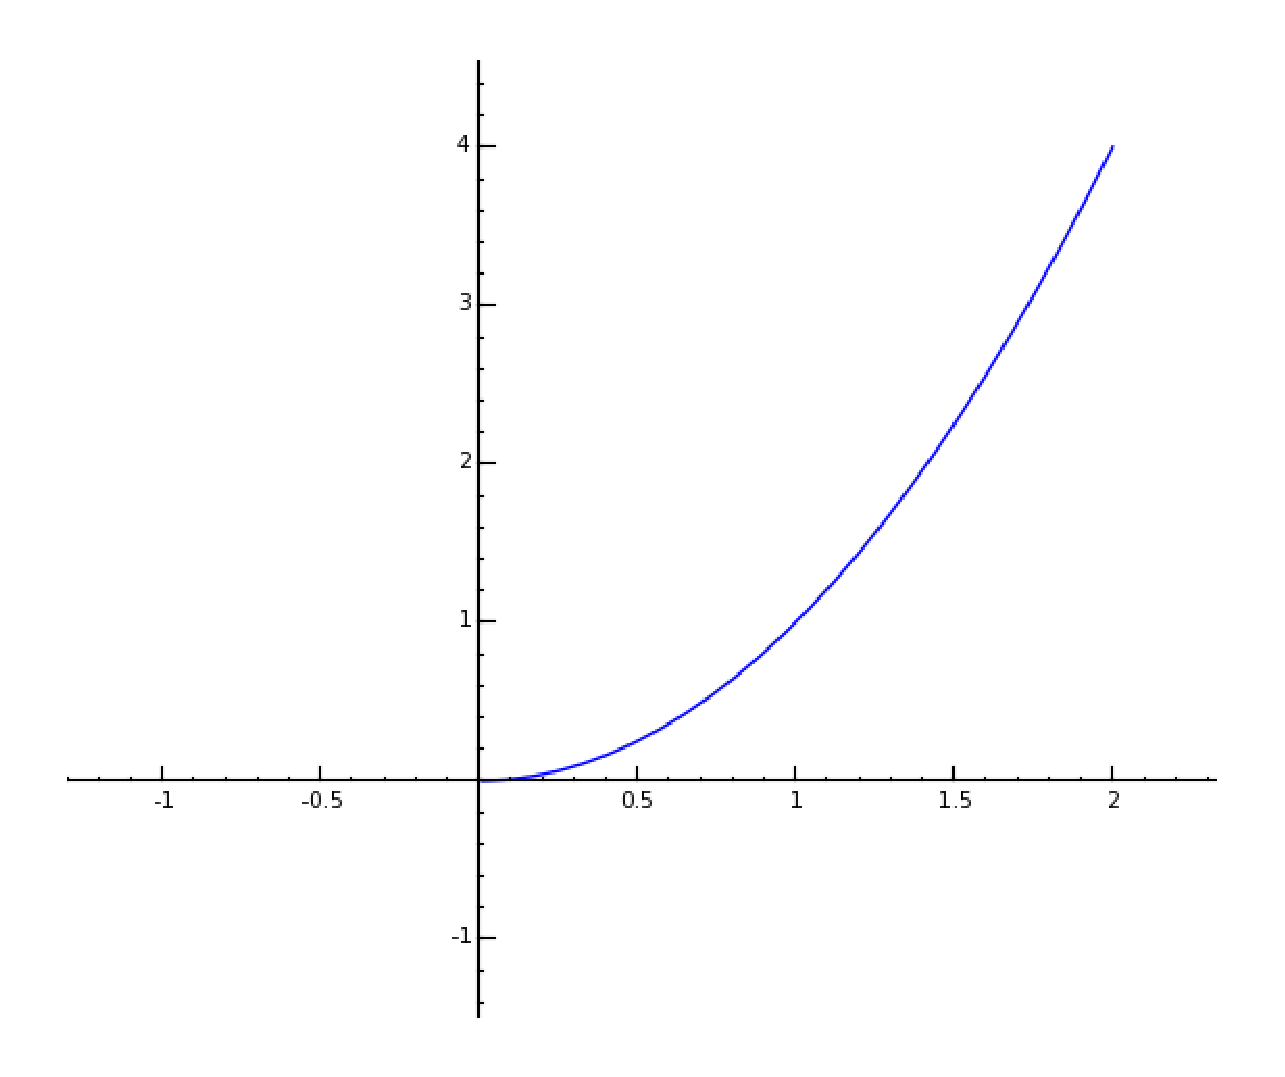
\includegraphics[height=5cm,width=5cm]{fcn-x2.eps}
\end{center}
\end{minipage}
\caption{The function $f(x)=x^2$.}
\label{fig:fcn-x2}
\end{figure}


Now flip this graph about the $45^o$ line:

\newpage

\begin{figure}[h!]
%\begin{tabular}{cc}
\begin{minipage}{\textwidth}
\begin{center}
%\vspace{1.0 cm}
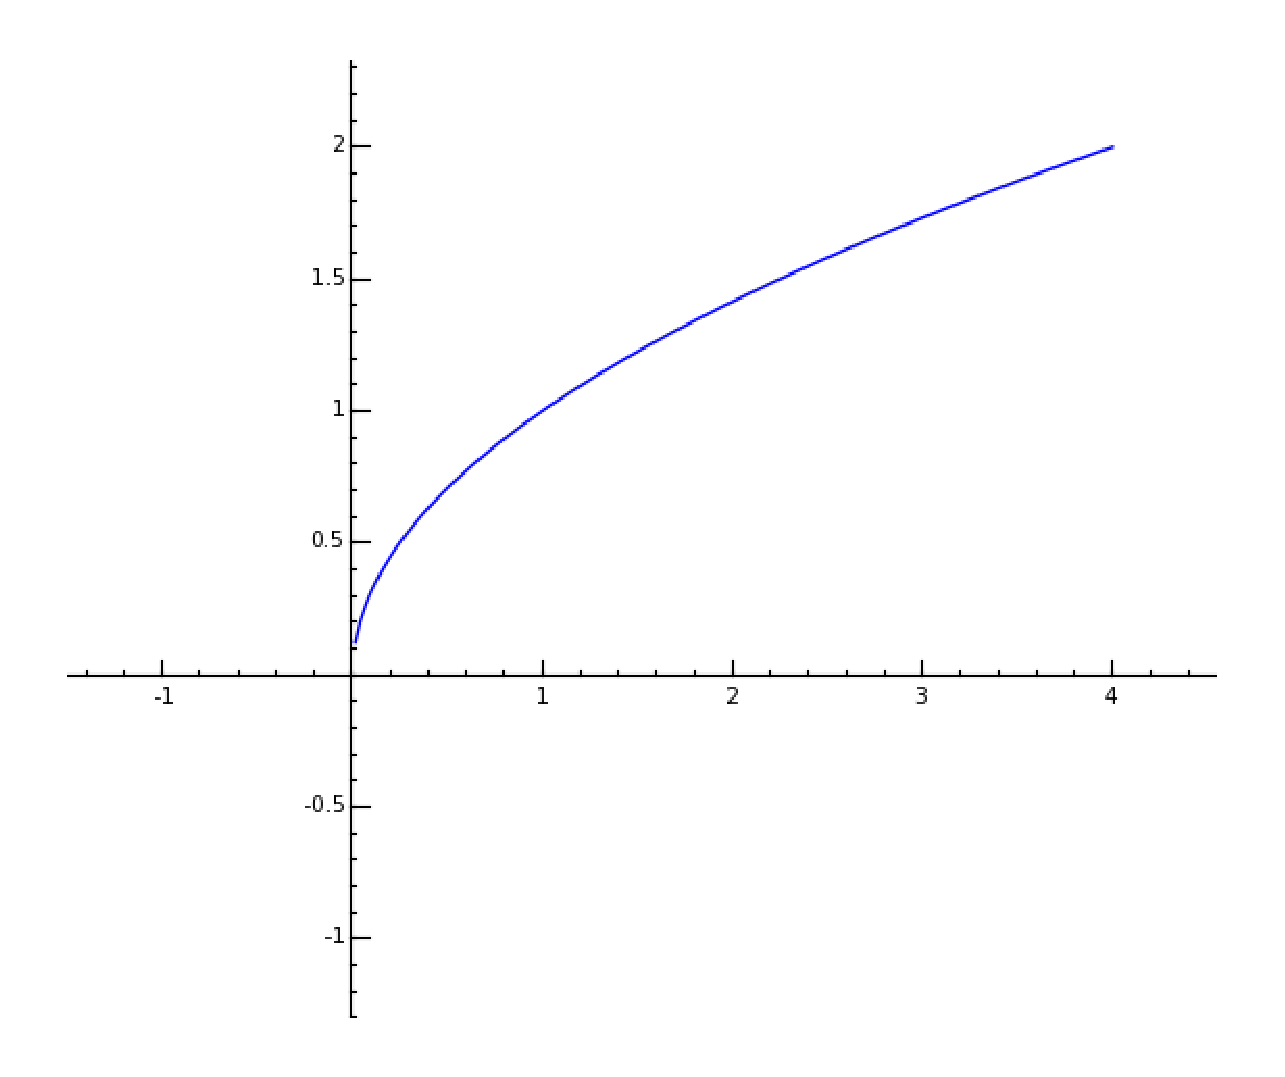
\includegraphics[height=5cm,width=5cm]{invfcn-x2.eps}
\end{center}
%\end{tabular}
\end{minipage}
\caption{The function $\phi(y)=f^{-1}(y)=\sqrt{y}$.}
\label{fig:invx2}
\end{figure}

The graph of inverse trig functions, for example,
$\tan(x)$ and $\arctan(x)$, are related in the same way.
}
\end{example}


Let us now differentiate the inverse functions

\[
   y = f(x)\ \ {\rm and}\ \  x = \phi(y)
\]
simultaneously by the General Rule.

\begin{itemize}
\item  
FIRST STEP. $	y + \Delta y 	= f(x + \Delta x)$, $	x + \Delta x =\phi(y + \Delta y)$
\item  
SECOND STEP. 
\[
\begin{array}{rlcrl}
y + \Delta y &	= f(x + \Delta x),  & \qquad & 	x + \Delta x &=	\phi (y + \Delta y)\\
  	y &= f(x),  & \qquad &	x &=\phi (y)\\
\Delta y &= f(x + \Delta x) - f(x), & \qquad &	\Delta x &= \phi(y + \Delta y) - \phi (y)\\
\end{array}
\]

\item  
THIRD STEP. 
\[
\frac{\Delta y}{\Delta x} = \frac{f(x + \Delta x) - f(x)}{\Delta x},
\qquad
\frac{\Delta x}{\Delta y} = \frac{\phi(y + \Delta y) - \phi(y)}{\Delta y}.
\]
Taking the product of the left-hand forms of these ratios, we get
$\frac{\Delta y}{\Delta x} \cdot \frac{\Delta x}{\Delta y} 	= 1$,
or, 	$\frac{\Delta y}{\Delta x} 	= \frac{1}{\frac{\Delta x}{\Delta y}}$.

\item  
FOURTH STEP. Passing to the limit,

\begin{equation}
%(C) 
	\frac{dy}{dx} 	= \frac{1}{\frac{dx}{dy}},
\label{eqn:C-43}
\end{equation}
or,

\[
%(D) 
	f'(x) 	= \frac{1}{\phi'(y)}.
\]
\end{itemize}

{\it The derivative of the inverse function is equal to the reciprocal 
of the derivative of the direct function.}


%44. 
\section{Differentiation of a logarithm}
\label{sec:44}

Let\footnote{The student must not forget that this function is defined 
only for positive values of the base $a$ and the variable $v$.}
$y = log_av$.

Differentiating by the General Rule %p. 29 [§ 31], 
(\S \ref{sec:31}), % new
considering $v$ as the independent variable, we have

\begin{itemize}
\item 
FIRST STEP. $	\ y + \Delta y 	= \log_a(v + \Delta v)$ .
\item 
SECOND STEP\footnote{If we take the third and fourth steps 
without transforming the right-hand member, there results:

Third step: $\frac{\Delta y}{\Delta v} 
= \frac{\log_a(v + \Delta v) - \log_a v}{\Delta v}$.

Fourth step. $\frac{dy}{dx} = \frac{0}{0}$, which is indeterminate. 

Hence the limiting value of the right-hand member in the third step cannot be 
found by direct substitution, and the above transformation is necessary.}.

\[
\begin{array}{ll}
 \Delta y &= \log_a(v + \Delta v) - \log_a v\\
 & = \log_a \left ( \frac{v + \Delta v}{v} \right )\\
& = \log_a \left ( 1 + \frac{\Delta v}{v} \right ).
\end{array}
\]
by item (8), \S \ref{sec:1}.

\item 
THIRD STEP. 
\[
\begin{array}{ll}
\frac{\Delta y}{\Delta x} &= \frac{1}{\Delta v} 
\log_a \left ( 1 + \frac{\Delta v}{v} \right ) \\
&= \log_a \left ( 1 + \frac{\Delta v}{v} \right )^{\frac{1}{\Delta v}}\\
 & 	= \frac{1}{v} 
\log_a \left ( 1 + \frac{\Delta v}{v} \right )^{\frac{v}{\Delta v}}.
\end{array}
\]
[Dividing the logarithm by $v$ and at the same 
time multiplying the exponent of the 
parenthesis by $v$ changes the form of the expression but not its value (see 
item (9), \S \ref{sec:1}.]

\item 
FOURTH STEP. $	\frac{dy}{dv} 	= \frac{1}{v} \log_a e$.
[When $\Delta v \to 0$ $\frac{\Delta v}{v} \to 0$. Therefore 
$\lim_{\Delta v \to 0} 
\left ( 1 + \frac{\Delta v}{v} \right )^{\frac{v}{\Delta v}} = e$, 
from \S \ref{sec:23}, placing $x = \frac{\Delta v}{v}$.]
\end{itemize}

Hence

\begin{equation}
%(A) 	
\frac{dy}{dv} 	= \frac{d}{dv} \left ( \log_a v \right ) 
= \log_a e \cdot \frac{1}{v}.
\label{eqn:A-44}
\end{equation}
Since $v$ is a function of $x$ and it is required to differentiate $\log_a v$ 
with respect to $x$, we must use formula (\ref{eqn:A-42}),
for differentiating a function of a function, namely,
\[
  	\frac{dy}{dx} 	= \frac{dy}{dv} \cdot \frac{dv}{dx}.
\]
Substituting 
the % new
value of $\frac{dy}{dv}$ from (\ref{eqn:A-44}), we get
\[
  	\frac{dy}{dx} 	= \log_a e \cdot \frac{1}{v} \cdot \frac{dv}{dx}.
\]
Therefore, $\frac{d}{dx} (\log_a x) 	
= \log_s e \cdot \frac{\frac{dv}{dx}}{v}$
(equation (VIII) above).
When $a = e$,\ $\log_a e = log_e e = 1$, and (VIII) becomes
$\frac{d}{dx} (\log v) 	= \frac{\frac{dv}{dx}}{v}$ (equation (VIIIa) above).

The derivative of the logarithm of a function is equal to the product of 
the modulus\footnote{The logarithm of $e$ to any base $a$ ( $= log_ae$) is 
called the {\it modulus} of the system whose base is $a$. In Algebra it is 
shown that we may find the logarithm of a number $N$ 
to any base $a$ by means of the formula
$
    \log_a N = \log_a e \cdot \log_e N = \frac{\log_e N}{\log_e a}.
$
The modulus of the common or Briggs system with base $10$ is
$\log_{10}e = .434294...$.}
of the system of logarithms and the derivative of the function, 
divided by the function.

\vskip .2in

\begin{Verbatim}[fontsize=\footnotesize,fontfamily=courier,fontshape=tt,frame=single,label=\sage]

sage: t = var('t')
sage: f = function('f', t)
sage: log(f(t)).diff(t)
diff(f(t), t, 1)/f(t)
sage: f = lambda x: 1-x^2
sage: log(f(t)).diff(t)
-2*t/(1 - t^2)

\end{Verbatim}

%45. 
\section{Differentiation of the simple exponential function}

Let $y 	= a^v$, \qquad $a > 0$.
Taking the logarithm of both sides to the base $e$, we get
$\log y = v \log a$,
or $v 	= \frac{\log y}{\log a}	= \frac{1}{\log a} \cdot \log y$.
Differentiate with respect to $y$ by formula (VIIIa),

\[
  	\frac{dv}{dy} 	= \frac{1}{\log a} \cdot \frac{1}{y};
\]
and from (\ref{eqn:C-43}),relating to inverse functions, we get
$  	\frac{dy}{dv} 	= \log a \cdot y$,
or,
\[
%(A)
 	\frac{dy}{dv} 	= \log a \cdot a^v.
\]
Since $v$ is a function of $x$ and it is required to differentiate 
$a^v$ with respect to $x$, we must use formula (\ref{eqn:A-42}), 
for differentiating a function of a function, namely,
\[
  	\frac{dy}{dx} 	= \frac{dy}{dv} \cdot \frac{dv}{dx}.
\]
Substituting the value of $\frac{dy}{dx}$ from %(A)
above, % new
we get
\[
  	\frac{dy}{dx} 	= \log a \cdot a^v \cdot \frac{dv}{dx}.
\]
Therefore, $\frac{d}{dx} (a^v) 	= \log a \cdot a^v \cdot \frac{dv}{dx}$
(equation (IX) in \S \ref{sec:33}  above).

\vskip .2in

\begin{Verbatim}[fontsize=\footnotesize,fontfamily=courier,fontshape=tt,frame=single,label=\sage]

sage: t = var('t')
sage: f = lambda x: x^2
sage: f = function('f', t)
sage: (3^f(t)).diff(t)
log(3)*3^f(t)*diff(f(t), t, 1)
sage: f = lambda x: x^7
sage: (3^f(t)).diff(t)
7*log(3)*t^6*3^t^7

\end{Verbatim}
\vskip .2in


When $a = e$,\ $\log a = \log e = 1$, and (IX) becomes
$\frac{d}{dx} (e^v) 	= e^v \frac{dv}{dx}$ (equation (IXa) in \S \ref{sec:33} above) .

{\it The derivative of a constant with a variable exponent is equal to the 
product of the natural logarithm of the constant, the constant with the 
variable exponent, and the derivative of the exponent.}

\vskip .2in

\begin{Verbatim}[fontsize=\footnotesize,fontfamily=courier,fontshape=tt,frame=single,label=\sage]

sage: t = var('t')
sage: f = lambda x: x^2
sage: f = function('f', t)
sage: (3^f(t)).diff(t)
log(3)*3^f(t)*diff(f(t), t, 1)
sage: f = lambda x: x^7
sage: (3^f(t)).diff(t)
7*log(3)*t^6*3^t^7

\end{Verbatim}
\vskip .2in

%46. 
\section{Differentiation of the general exponential function}
\label{sec:46}

Let\footnote{Here $u$ can assume only positive values.}
$ y 	= u^v$.
Taking the logarithm of both sides to the base $e$,
$\log_e y= v \log_e u$, or, $y 	= e^{v \log u}$.

Differentiating by formula (IXa),

\[
\begin{array}{ll}
  	\frac{dy}{dx} &	= e^{v \log u} \frac{d}{dx} (v \log u)\\
  &	= e^{v \log u} \left ( \frac{v}{u} \frac{du}{dx} + \log u \frac{dv}{dx} \right ) \ \ {\rm by\ V}\\
  &	= u^v \left ( \frac{v}{u} \frac{du}{dx} + \log u \frac{dv}{dx} \right )
\end{array}
\]
Therefore, $\frac{d}{dx}(u^v) 	= vu^{v - 1}\frac{du}{dx} + \log u \cdot u^v \frac{dv}{dx}$
(equation (X) in \S \ref{sec:33}  above).

{\it The derivative of a function with a variable exponent is equal to the 
sum of the two results obtained by first differentiating by (VI), 
regarding the exponent as constant, and again differentiating by (IX), 
regarding the function as constant.}

Let $v = n$, any constant; then (X) reduces to

\[
    \frac{d}{dx}(u^n) = nu^{n - 1} \frac{du}{dx}.
\]
But this is the form differentiated in \S \ref{sec:40}; %§ 40
therefore (VI) holds true for any value of $n$.

\begin{example}
{\rm
Differentiate $y = \log(x^2 + a)$.

Solution. 	

\[
\begin{array}{ll}
\frac{dy}{dx} 	&= \frac{\frac{d}{dx}(x^2 + a)}{x^2 + a} \ \ {\rm by\ VIIIa}\ (v = x^2 + a)\\
  	&= \frac{2x}{x^2 + a} .
\end{array}
\]
}
\end{example}

\begin{example}
\label{ex:2-46}
{\rm
Differentiate $y = \log \sqrt{1 - x^2}$.


Solution. 

\[
\begin{array}{ll}
	\frac{dy}{dx} 
&	= \frac{\frac{d}{dx}(1 - x^2)^{\frac{1}{2}}}{(1 - x^2)^{\frac{1}{2}}} \ \ {\rm by\ VIIIa}\\
&  	= \frac{\frac{1}{2} (1 - x^2)^{-\frac{1}{2}}(-2x)}{(1 - x^2)^{\frac{1}{2}}} \ \ {\rm by\ VI}\\
&  	= \frac{x}{x^2 - 1}.
\end{array}
\]
}
\end{example}

\begin{example}
{\rm
Differentiate $y = a^{3x^2}$.

Solution.

\[
\begin{array}{ll}
 	\frac{dy}{dx} &	= \log a \cdot a^{3x^2} \frac{d}{dx}(3 x^2) \ \ {\rm by\ IX}\\
  &	= 6x \log a \cdot a^{3x^2}.
\end{array}
\]
}
\vskip .2in

\begin{Verbatim}[fontsize=\footnotesize,fontfamily=courier,fontshape=tt,frame=single,label=\sage]

sage: t,a = var('t,a')
sage: f = lambda x: 3*x^2
sage: (a^f(t)).diff(t)
6*a^(3*t^2)*log(a)*t

\end{Verbatim}
\vskip .2in

\end{example}

\begin{example}
{\rm
Differentiate $y = be^{c^2 + x^2}$.

Solution. 

\[
\begin{array}{ll}
	\frac{dy}{dx} 
&=	b\frac{d}{dx} \left ( e^{c^2 + x^2} \right ) \ \ {\rm by\ IV}\\
&  	= be^{c^2 + x^2} \frac{d}{dx} (c^2 + x^2)  \ \ {\rm by\ IXa}\\
&  	= 2bxe^{c^2 + x^2}.
\end{array}
\]
}
\end{example}

\begin{example}
\label{ex:5-46}
{\rm
Differentiate $y = x^{e^x}$.

Solution.

\[
\begin{array}{ll}
	\frac{dy}{dx} 
&	= e^x x^{e^x - 1} \frac{d}{dx} (x) + x^{e^x} \log x \frac{d}{dx} (e^x)  \ \ {\rm by\ X}\\
&  	= e^x x^{e^x - 1} + x^{e^x} \log x \cdot e^x\\
&  	= e^x x^{e^x} \left ( \frac{1}{x} + \log x \right ) 
\end{array}
\]
}
\end{example}

%47. 
\section{Logarithmic differentiation}

Instead of applying (VIII) and (VIIIa) at once in differentiating logarithmic 
functions, we may sometimes simplify the work by first making use of one 
of the formulas 7-10 in \S \ref{sec:1}. %on p. 1 [§ 1]. 
Thus above Illustrative Example \ref{ex:2-46} may be solved as follows:


\begin{example}
{\rm
Differentiate $y = \log \sqrt{1 - x^2}$.

Solution. By using 10, in \S \ref{sec:1}, %p. 1, 
we may write this in a form free from radicals as follows:
$  	y 	= \frac{1}{2} \log (1 - x^2)$.
Then 
\[
\begin{array}{ll}
	\frac{dy}{dx} 	
&= \frac{1}{2} \frac{\frac{d}{dx} (1 - x^2)}{1 - x^2}  \ \ {\rm by\ VIIIa}\\
&  	= \frac{1}{2} \cdot \frac{-2}{1 - x^2} = \frac{x}{x^2 - 1}. 
\end{array}
\]
}
\end{example}

\begin{example}
{\rm
Differentiate $y = \log \sqrt{\frac{1 + x^2}{1 - x^2}}$.

Solution. Simplifying by means of 10 and 8, in \S \ref{sec:1}, %p. 1 [§ 1],

\[
\begin{array}{ll}
  	y 	&= \frac{1}{2} [ \log (1 + x^2) - \log (1 - x^2) ]\\
\frac{dy}{dx} 	
&= \frac{1}{2} \left [ \frac{\frac{d}{dx} (1 + x^2)}{1 + x^2} 
- \frac{\frac{d}{dx} (1 - x^2)}{1 - x^2} \right ]   \ \ {\rm by\ VIIIa,\ etc.}\\
&  	= \frac{x}{1 + x^2} + \frac{x}{1 - x^2} = \frac{2x}{1 - x^4}. 
\end{array}
\]
}
\end{example}

In differentiating an exponential function, especially a variable 
with a variable exponent, the best plan is first to take the logarithm of 
the function and then differentiate. Thus Example \ref{ex:5-46} %   Illustrative Example 5, p. 50 [§ 46], 
is solved more elegantly as follows:

\begin{example}
{\rm
Differentiate $y = x^{e^x}$.

Solution. Taking the logarithm of both sides, $\log y = e^x\log x$, by 9 in \S \ref{sec:1}.
%	By 9, p. 1 [§ 1]
Now differentiate both sides with respect to $x$:

\[
\begin{array}{ll}
\frac{\frac{dy}{dx}}{y} 
&	= e^x \frac{d}{dx} (\log x) + \log x \frac{d}{dx} (e^x)   \ \ {\rm by\ VIII\ and\ V}\\
&  	= e^x \cdot \frac{1}{x} + \log x \cdot e^x,
\end{array}
\]
or, 	

\[
\frac{dy}{dx} 	= e^x \cdot y \left ( \frac{1}{x} \log x \right )
  	= e^x x^{e^x} \left ( \frac{1}{x} + \log x \right ).
\]
}
\end{example}

\begin{example}
{\rm
Differentiate $y = (4x^2 - 7)^{2 + \sqrt{x^2 - 5}}$.

Solution. Taking the logarithm of both sides,

\[
    \log y = (2 + \sqrt{x^2 - 5}) \log (4x^2 - 7).
\]
Differentiating both sides with respect to $x$,

\[
    \frac{1}{y} \frac{dy}{dx} 	= (2 + \sqrt{x^2 - 5}) \frac{8x}{4x^2 - 7} + \log(4x^2 - 7) \cdot \frac{x}{\sqrt{x^2 - 5}}.
\]
\[
    \frac{dy}{dx} 	= x(4x^2 - 7)^{2 + \sqrt{x^2 - 5}} \left [ \frac{8(2 + \sqrt{x^2 - 5})}{4x^2 - 7} + \frac{\log (4x^2 - 7)}{\sqrt{x^2 - 5}} \right ]. 
\]
}
\end{example}

In the case of a function consisting of a number of factors it is sometimes 
convenient to take the logarithm before differentiating. Thus,

\begin{example}
{\rm
Differentiate $y = \sqrt{\frac{(x - 1)(x - 2)}{(x - 3)(x - 4)}}$.

Solution. Taking the logarithm of both sides,

\[
    \log y = \frac{1}{2} [\log (x -1) + \log (x - 2) - \log(x - 3) - \log(x - 4)].
\]
Differentiating both sides with respect to $x$,

\[
\begin{array}{ll}
\frac{1}{y} \frac{dy}{dx} &= \frac{1}{2} \left [ \frac{1}{x - 1} + \frac{1}{x - 2} - \frac{1}{x - 3} - \frac{1}{x - 4} \right ]\\
&	= -\frac{2x^2 - 10x + 11}{(x - 1)(x - 2)(x - 3)(x - 4)},
\end{array}
\]
or, 

\[
\frac{dy}{dx} 	= -\frac{2x^2 - 10x - 11}{(x - 1)^{\frac{1}{2}} (x - 2)^{\frac{1}{2}} ( x - 3)^{\frac{3}{2}} (x - 4)^{\frac{3}{2}}}.
\]
}
\end{example}

\section{Examples}

Differentiate the following\footnote{Though the answers are given 
below, it may be that your computation differs from the solution given.
You should then try to show algebraically that your form is that same 
as that given.}: %% new footnote

\begin{enumerate}

\item
%1
$y = \log(x + a)$\qquad\qquad\qquad\qquad\qquad\qquad Ans: 	$\frac{dy}{dx} = \frac{1}{x + a}$

\item
%2
$y = \log(ax + b)$\qquad\qquad\qquad\qquad\qquad\qquad Ans: 	$\frac{dy}{dx} = \frac{a}{ax + b}$

\item
%3
$y = \log \frac{1 + x^2}{1 - x^2}$\qquad\qquad\qquad\qquad\qquad\qquad Ans: 	$\frac{dy}{dx} = \frac{4x}{1 - x^4}$

\item
%4
$y = \log(x^2 + x)$\qquad\qquad\qquad\qquad\qquad\qquad Ans: 	$y' = \frac{2x + 1}{x^2 + x}$

\item
%5
$y = \log(x^3 - 2x + 5)$\qquad\qquad\qquad\qquad\qquad\qquad Ans: 	$y' = \frac{3x^2 - 2}{x^3 - 2x + 5}$

\item
%6
$y = \log_a(2x + x^3)$\qquad\qquad\qquad\qquad\qquad\qquad Ans: 	$y' = \log_a e \cdot \frac{2 + 3x^2}{2x + x^3}$

\item
%7
$y = x\log x$\qquad\qquad\qquad\qquad\qquad\qquad Ans: 	$y' = \log x + 1$

\item
%8
$f(x) = \log (x^3)$\qquad\qquad\qquad\qquad\qquad\qquad Ans: 	$f'(x) = \frac{3}{x}$

\item
%9
$f(x) = \log^3 x$\qquad\qquad\qquad\qquad\qquad\qquad Ans: 	$f'(x) = \frac{3 \log^2 x}{x}$

(Hint: $\log^3x = (\log x)^3$. Use first VI, $v = \log x$, $n = 3$; and then VIIIa.)

\item
%10
$f(x) = \log \frac{a + x}{a - x}$\qquad\qquad\qquad\qquad\qquad\qquad Ans: 	$f'(x) = \frac{2a}{a^2 - x^2}$

\item
%11
$f(x) = \log (x + \sqrt{1 + x^2})$\qquad\qquad\qquad\qquad\qquad\qquad Ans: 	$f'(x) = \frac{1}{\sqrt{1 + x^2}}$

\item
%12
$\frac{d}{dx} e^{ax} = ae^{ax}$

\item
%13
$\frac{d}{dx} e^{4x + 5} = 4e^{4x + 5}$

\item
%14
$\frac{d}{dx} a^{3x} = 3a^{3x} \log a$

\item
%15
$\frac{d}{dt} \log(3 - 2t^2) = \frac{4t}{2t^2 - 3}$

\item
%16
$\frac{d}{dy} \log \frac{1 + y}{1 - y} = \frac{2}{1 - y^2}$

\item
%17
$\frac{d}{dx}e^{b^2 + x^2} = 2xe^{b^2 + x^2}$

\item
%18
$\frac{d}{d\theta} a^{\log a} = \frac{1}{\theta} a^{\log \theta} \log a$

\item
%19
$\frac{d}{ds}b^{s^2} = 2x \log b \cdot b^{s^2}$

\item
%20
$\frac{d}{dv} ae^{\sqrt{v}} = \frac{ae^{\sqrt{v}}}{2\sqrt{v}}$

\item
%21
$\frac{d}{dx} a^{e^x} = \log a \cdot a^{e^x} \cdot e^x$

\item
%22
$y = 7^{x^2 + 2x}$\qquad\qquad\qquad\qquad\qquad\qquad Ans: 	$y' = 2\log 7 \cdot (x + 1) 7^{x^2 + 2x}$

\item
%23
$y = c^{a^2 - x^2}$\qquad\qquad\qquad\qquad\qquad\qquad Ans: 	$y' = -2x \log c \cdot c^{a^2 - x^2}$

\item
%24
$y = \log \frac{e^x}{1 + e^x}$\qquad\qquad\qquad\qquad\qquad\qquad Ans: 	$\frac{dy}{dx} = \frac{1}{1 + e^x}$

\item
%25
$\frac{d}{dx} \left [ e^x ( 1- x^2 \right ] = e^x (1 - 2x - x^2)$

\item
%26
$\frac{d}{dx} \left ( \frac{e^x - 1}{e^x + 1} \right ) = \frac{2e^x}{(e^x + 1)^2}$

\item
%27
$\frac{d}{dx} \left ( x^2 e^{ax} \right ) = xe^{ax}(ax + 2)$

\item
%28
$y = \frac{a}{2} (e^{\frac{x}{a}} - e^{-\frac{x}{a}})$\qquad\qquad\qquad\qquad\qquad\qquad Ans: 	
$\frac{dy}{dx} = \frac{1}{2} (e^{\frac{x}{a}} + e^{-\frac{x}{a}})$

\item
%29
$y = \frac{e^x - e^{-x}}{e^x + e^{-x}}$\qquad\qquad\qquad\qquad\qquad\qquad Ans: 	$\frac{dy}{dx} = \frac{4}{(e^x + e^{-x}))^2}$

\item
%30
$y = x^na^x$\qquad\qquad\qquad\qquad\qquad\qquad Ans: 	$y' = a^xx^{n - 1}(n + x\log a)$

\item
%31
$y = x^x$\qquad\qquad\qquad\qquad\qquad\qquad Ans: 	$y' = x^x(\log x + 1)$
\item
%32
$y = x^{\frac{1}{x}}$
\qquad\qquad\qquad\qquad\qquad\qquad Ans: 
$y' = \frac{x^{\frac{1}{x}} (1 - \log x)}{x^2}$

\item
%33
$y = x^{\log x}$\qquad\qquad\qquad\qquad\qquad\qquad Ans: 	$y' = \log (x^2) \cdot x^{\log x - 1}$
%sage: diff(x^(log(x)),x)
%2*x^(log(x) - 1)*log(x)

\item
%34
$f(y) = \log y \cdot e^y$\qquad\qquad\qquad\qquad\qquad\qquad Ans: 	$f'(y) = e^y \left ( \log y + \frac{1}{y} \right )$

\item
%35
$f(s) = \frac{\log s}{e^s}$\qquad\qquad\qquad\qquad\qquad\qquad Ans: 	$f'(s) = \frac{1 - s \log s}{s e^s}$

\item
%36
$f(x) = \log(\log x)$\qquad\qquad\qquad\qquad\qquad\qquad Ans: 	$f'(x) = \frac{1}{x \log x}$

\item
%37
$F(x) = \log^4(\log x)$\qquad\qquad\qquad\qquad\qquad\qquad Ans: 	$F'(x) = \frac{4 \log^3 (\log x)}{x \log x}$

\item
%38
$\phi (x) = \log(\log^4x)$\qquad\qquad\qquad\qquad\qquad\qquad Ans: 	$\phi'(x) = \frac{4}{x \log x}$

\item
%39
$\psi(y) = \log \sqrt{\frac{1 + y}{1 - y}}$\qquad\qquad\qquad\qquad\qquad\qquad Ans: 	$\psi'(y) = \frac{1}{1 - y^2}$

\item
%40
$f(x) = \log \frac{\sqrt{x^2 + 1} - x}{\sqrt{x^1 + 1} + x}$\qquad\qquad\qquad\qquad\qquad\qquad Ans: 	$f'(x) = -\frac{2}{\sqrt{1 + x^2}}$

\item
%41
$y = x^{\frac{1}{\log x}}$\qquad\qquad\qquad\qquad\qquad\qquad Ans: 	$\frac{dy}{dx} = 0$

\item
%42
$y = e^{x^x}$\qquad\qquad\qquad\qquad\qquad\qquad Ans: 	$\frac{dy}{dx} = e^{x^x}(1 + \log x)x^x$

\item
%43
$y = \frac{c^x}{x^x}$\qquad\qquad\qquad\qquad\qquad\qquad Ans: 	
$\frac{dy}{dx} = \left ( \frac{c}{x} \right )^x \left ( \log \frac{c}{x} - 1 \right )$

\item
%44
$y = \left ( \frac{x}{n} \right )^{nx}$\qquad\qquad\qquad\qquad\qquad\qquad Ans: 	
$\frac{dy}{dx} = n \left ( \frac{x}{n} \right )^{nx} \left ( 1 + \log \frac{x}{n} \right )$

\item
%45
$w = v^{e^v}$\qquad\qquad\qquad\qquad\qquad\qquad Ans: 	
$\frac{dw}{dv} = v^{e^v} e^v \left ( \frac{1 + v \log v}{v} \right )$

\item
%46
$z = \left ( \frac{a}{t} \right )^t$\qquad\qquad\qquad\qquad\qquad\qquad Ans: 	$\frac{dz}{dt} 
= \left ( \frac{a}{t} \right )^t (\log a - \log t - 1)$

\item
%47
$y = x^{x^n}$\qquad\qquad\qquad\qquad\qquad\qquad Ans: 	$\frac{dy}{dx} = x^{x^n + n - 1}(n \log x + 1)$

\item
%48
$y = x^{x^x}$\qquad\qquad\qquad\qquad\qquad\qquad Ans: 	$\frac{dy}{dx} = x^{x^x} x^x \left ( \log x + \log^2 x + \frac{1}{x} \right )$

\item
%49
$y = a^{\frac{1}{\sqrt{a^2 - x^2}}}$\qquad\qquad\qquad\qquad\qquad\qquad Ans: 	$\frac{dy}{dx} = \frac{xy \log a}{(a^2 - x^2)^{\frac{3}{2}}}$

\item
%50
%Differentiate the following functions:
Compute the following derivatives: %% new

\[
\begin{array}{lll}
(a)\ \  \frac{d}{dx} x^2 \log x &  	(f)\ \  \frac{d}{dx} e^x \log x &  	(k)\ \  \frac{d}{dx} \log (a^x + b^x) \\
(b)\ \  \frac{d}{dx} (e^{2x} - 1)^4 &  	(g)\ \  \frac{d}{dx} x^3 3^x &	(l)\ \  \frac{d}{dx} \log_10 (x^2 + 5x)\\
(c)\ \  \frac{d}{dx} \log \frac{3x + 1}{x + 3} &  	(h)\ \  \frac{d}{dx} \frac{1}{x \log x} &  	(m)\ \  \frac{d}{dx} \frac{2 + x^2}{e^{3x}}\\
(d)\ \  \frac{d}{dx} \log \frac{1 - x^2}{\sqrt{1 + x}} &  	(i)\ \  \frac{d}{dx} \log x^3 \sqrt{1 + x^2} &  	(n)\ \  \frac{d}{dx} (x^2 + a^2) e^{x^2 + a^2}\\
(e)\ \  \frac{d}{dx} x^{\sqrt{x}} &  	(j)\ \  \frac{d}{dx} \left ( \frac{1}{x} \right )^x &  	(o)\ \  \frac{d}{dx} (x^2 + 4)^x.
\end{array}
\]

\item
%51
$y = \frac{(x + 1)^2}{(x + 2)^3 (x + 3)^4}$
\qquad\qquad\qquad\qquad\qquad\qquad Ans: 
 	$\frac{dy}{dx} = -\frac{(x + 1)(5x^2 + 14x + 5)}{(x + 2)^4 (x + 3)^5}$

\item
%52
$y = \frac{((x - 1)^{\frac{5}{2}}}{(x - 2)^{\frac{3}{4}}(x - 3)^{\frac{7}{3}}}$\qquad\qquad\qquad\qquad\qquad\qquad Ans: 	
$\frac{dy}{dx} 
= -\frac{(x - 1)^{\frac{3}{2}}(7x^2 + 30x - 97)}{12(x - 2)^{\frac{7}{4}}(x - 3)^{\frac{10}{3}}}$

\item
%53
$y = x \sqrt{1 - x} (1 + x)$
\qquad\qquad\qquad\qquad\qquad\qquad Ans: 
 	$\frac{dy}{dx} = \frac{2 + x - 5x^2}{2\sqrt{1 - x}}$

\item
%54
$y = \frac{x(1 + x^2)}{\sqrt{1 - x^2}}$ 
	\qquad\qquad\qquad\qquad\qquad\qquad Ans: 
$\frac{dy}{dx} = \frac{1 + 3x^2 - 2x^4}{(1 - x^2}^{\frac{3}{2}}$

\item
%55
$y = x^5(a + 3x)^3(a - 2x)^2$\qquad\qquad\qquad
{\scriptsize{Ans: 	
$\frac{dy}{dx} = 5x^4(a + 3x)^2(a - 2x)(a^2 + 2ax - 12x^2)$}}

\end{enumerate}


%48. 
\section{Differentiation of $\sin v$}

Let 	$y 	= \sin v$.
By General Rule, \S \ref{sec:31}, %p. 29 [§ 31], 
considering $v$ as the independent variable, we have

\begin{itemize}

\item
FIRST STEP. 	$y + \Delta y 	= \sin(v + \Delta v)$.

\item
SECOND STEP\footnote{If we take the third and fourth steps without 
transforming the right-hand member, there results:

Third step. $\frac{\Delta y}{\Delta v} = \frac{\sin(v + \Delta v) - \sin v}{\Delta v}$

Fourth step. $\frac{dy}{dv} = \frac{0}{0}$, which is indeterminate (see footnote, \S \ref{sec:44}).
%p. 46 [§ 44]).
}
\footnote{Let 	$A 	= v + \Delta v$ % 	  	A 	= v + \Delta v
and 	$B 	= v$. % 	  	B 	= v
Adding, 	$A + B 	= 2v + \Delta v$ and subtracting, $A - B 	= \Delta v$.
Therefore 	$\frac{1}{2}(A + B) 	= v + \frac{\Delta v}{2}$ and 
$\frac{1}{2}(A - B) 	= \frac{\Delta v}{2}$.
Substituting these values of $A$, $B$, $\frac{1}{2}(A + B)$, $\frac{1}{2}(A - B)$ in terms 
of $v$ and $\Delta v$ in the formula from Trigonometry (item 42 from \S \ref{sec:1}) %, p. 2 [§ 1]),
$
	\sin A - \sin B 	= 2 \cos \frac{1}{2} (A + B) \sin \frac{1}{2} (A - B),
$
we get 	

$
\sin (v + \Delta v) - \sin v 	= 2 \cos \left ( v + \frac{\Delta v}{2} \right ) \sin \frac{\Delta v}{2}.
$
}
\[
\Delta y 	= \sin(v + \Delta v) - \sin v
  	= 2 \cos \left ( v + \frac{\Delta v}{2} \right ) \cdot \sin \frac{\Delta v}{2}.
\]

\item
THIRD STEP. 	

\[
\frac{\Delta y}{\Delta v} 
= \cos \left ( v + \frac{\Delta v}{2} \right ) \left ( \frac{\sin \frac{\Delta v}{2}}{\frac{\Delta v}{2}} \right ).
\]
\item
FOURTH STEP. $\frac{dy}{dx} 	= \cos v$.

(Since $\lim_{\Delta v \to 0} \left ( \frac{\sin \frac{\Delta v}{2}}{\frac{\Delta v}{2}} \right ) = 1$, 
by \S \ref{sec:22}, %§ 22, p. 21, 
and $\lim_{\Delta v \to 0} \cos \left ( v + \frac{\Delta v}{2} \right ) = \cos v$.)

\end{itemize}

Since $v$ is a function of $x$ and it is required to differentiate $\sin v$ with respect to $x$, 
we must use formula (A), \S \ref{sec:42}, %§ 42, 
for differentiating a function of a function, namely,

\[
  	\frac{dy}{dx} 	= \frac{dy}{dv} \cdot \frac{dv}{dx}.
\]
Substituting value $\frac{dy}{dx}$ from Fourth Step, we get
$  	\frac{dy}{dx} 	= \cos v \frac{dv}{dx}$.
Therefore, 
\[
\frac{d}{dx} (\sin v) 	= \cos v \frac{dv}{dx}
\]
(equation (XI) in \S \ref{sec:33}  above).

The statement of the corresponding rules will now be left to the student.

%49. 
\section{Differentiation of $\cos v$}

Let $y 	= \cos v$.
By item 29, \S \ref{sec:1}, %p. 2 [§ 1], 
this may be written
\[
  	y 	= \sin \left ( \frac{\pi}{2} - v \right ).
\]
Differentiating by formula (XI),

\[
\begin{array}{ll}
  \frac{dy}{dx} 
& = \cos \left ( \frac{\pi}{2} - v \right ) \frac{d}{dx} \left ( \frac{\pi}{2} - v \right )\\
& = \cos \left ( \frac{\pi}{2} - v \right ) \left ( -\frac{dv}{dx} \right )\\
& = -\sin x \frac{dv}{dx}.
\end{array}
\]
(Since $\cos \left ( \frac{\pi}{2} \right ) = \sin v$, by 29, \S \ref{sec:1}.) %p. 2.]
Therefore, 

\[
\frac{d}{dx} (\cos v) 	= -\sin v \frac{dv}{dx},
\]
(equation (XII) in \S \ref{sec:33}  above).

\vskip .2in

\begin{Verbatim}[fontsize=\scriptsize,fontfamily=courier,fontshape=tt,frame=single,label=\sage]

sage: t = var('t')
sage: f = function('f', t)
sage: cos(f(t)).diff(t)
-sin(f(t))*diff(f(t), t, 1)

\end{Verbatim}


%50. 
\section{Differentiation of $\tan v$}

Let $y 	= \tan v$.
By item 27, \S \ref{sec:1}, %p. 2 [§ 1], 
this may be written

\[
\begin{array}{ll}
  	\frac{dy}{dx}
& 	= \frac{\cos v \frac{d}{dx}(\sin v) - \sin v \frac{d}{dx}(\cos v)}{\cos^2 v}\\
 & 	= \frac{\cos^2 v \frac{dv}{dx} + \sin^2 v \frac{dv}{dx}}{\cos^2 v}\\
 & 	= \frac{\frac{dv}{dx}}{\cos^2 v} = \sec^2 v \frac{dv}{dx}.
\end{array}
\]
Therefore, 

\[
\frac{d}{dx}(\tan x) 	= \sec^2 v \frac{dv}{dx},
\]
(equation (XIII) in \S \ref{sec:33}  above).


%51. 
\section{Differentiation of $\cot v$}

Let $y 	= \cot v$.
By item 26, \S \ref{sec:1}, %p. 2 [§ 1], 
this may be written $y 	= \frac{1}{\tan v}$.
Differentiating by formula VII,

\[
\begin{array}{ll}
  	\frac{dy}{dx}
& 	= - \frac{\frac{d}{dx}(\tan v)}{\tan^2 v}\\
&  	= -\frac{\sec^2 \frac{dv}{dx}}{\tan^2 v} \\
& = -\csc^2 v \frac{dv}{dx}.
\end{array}
\]
Therefore, 
\[
\frac{d}{dx}(\cot v) 	= -\csc^2 v \frac{dv}{dx}
\]
(equation (XIII) in \S \ref{sec:33}  above).

%52. 
\section{Differentiation of $\sec v$}

Let $y = \sec v$.
By item 26,  \S \ref{sec:1}, %p. 2 [§ 1], 
this may be written
$y 	= \frac{1}{\cos v}$.
Differentiating by formula VII,

\[
\begin{array}{ll}
\frac{dy}{dx} 
&	= -\frac{\frac{d}{dx}(\cos v)}{\cos^2 v}\\
&  	=\frac{\sin v \frac{dv}{dx}}{\cos^2 v}\\
&  	= \frac{1}{\cos v} \frac{\sin v}{\cos v} \frac{dv}{dx}\\
&  	= \sec v \tan v \frac{dv}{dx}.
\end{array}
\]
Therefore, 
\[
\frac{d}{dx}(\sec v) 	= \sec v \tan v \frac{dv}{dx}
\]
(equation (XV) in \S \ref{sec:33}  above).

%53. 
\section{Differentiation of $\csc\, v$}

Let $y 	= \csc\, v$.
By item 26, \S \ref{sec:1}, %p. 2 [§ 1], 
this may be written
\[
  	y 	= \frac{1}{\sin v}.
\]
Differentiating by formula VII,

\[
\begin{array}{ll}
\frac{dy}{dx} 
&	= -\frac{\frac{d}{dx}(\sin v)}{\sin^2 v}\\
 & 	= -\frac{\cos v \frac{dv}{dx}}{\sin^2 v}\\
  &	= -\csc v \cot v \frac{dv}{dx}.
\end{array}
\]
Therefore, 
\[
\frac{d}{dx}(\csc v) 	= - \csc v \cot v \frac{dv}{dx}
\]
(equation (XVI) in \S \ref{sec:33}  above).

%54. 
\section{Differentiation of $\vers\, v$}

Let $y 	= \vers\ v$.
By definition, %% new Trigonometry 
this may be written
\[
  	\ y 	= 1 - \cos v\ .
\]
Differentiating, $\frac{dy}{dx} 	= \sin v \frac{dv}{dx}$.
Therefore, $\frac{d}{dx}(\vers\, v) 	= \sin v \frac{dv}{dx}$
(equation (XVII) in \S \ref{sec:33}  above).

\section{Exercises}

In the derivation of our formulas so far it has been necessary to 
apply the General Rule, \S \ref{sec:31}, %p. 29 [§ 31] 
(i.e. the four steps), only for the following:

\vskip .2in
\begin{center}
\begin{tabular}{lcc}
III &	$\frac{d}{dx}(u + v - w) 	= \frac{du}{dx} + \frac{dv}{dx} - \frac{dw}{dx} $ &	Algebraic sum.\\
V &	$\frac{d}{dx}(uv) 	= u \frac{dv}{dx} + v \frac{du}{dx}.  $ &	Product.\\
VII &	$\frac{d}{dx} \left ( \frac{u}{v} \right ) 	= \frac{v \frac{du}{dx} - u \frac{dv}{dx}}{v^2}.  $ &	Quotient.\\
VIII &	$\frac{d}{dx}(\log_a v) 	= \log_a e \frac{\frac{dv}{dx}}{v}. $ & 	Logarithm.\\
XI &	$\frac{d}{dx}(\sin v) 	= \cos v \frac{dv}{dx} $ & 	Sine.\\
XXV &	$\frac{dy}{dx} 	= \frac{dy}{dv} \cdot \frac{dv}{dx}.  $ &	Function of a function.\\
XXVI &	$\frac{dy}{dx} 	= \frac{1}{\frac{dx}{dy}}.  $ &	Inverse functions.\\
\end{tabular}
\end{center}
\vskip .2in

Not only do all the other formulas we have deduced depend on these, but all 
we shall deduce hereafter depend on them as well. Hence it follows that the 
derivation of the fundamental formulas for differentiation involves the calculation 
of only two limits of any difficulty, viz.,

\[
  	\lim_{v \to 0} \frac{\sin v}{1} 	= 1\ \ \ \ \ \ {\rm by\ \S \ref{sec:22}},% § 22, p. 21
\]
and 

\[
\lim_{v \to 0}(1 + v)^{\frac{1}{v}} 	= e\  \ \ \ \ \ \ 	{\rm by\ \S \ref{sec:23}}. %By § 23, p. 22
\]

\vskip .3in
\noindent
{\bf Examples/exercises:}

Differentiate the following:

\begin{enumerate}
\item
%1. 
$y = \sin (ax^2)$ .

\[
\frac{dy}{dx} 	= \cos ax^2 \frac{d}{dx}(ax^2),\ \ \ {\rm  by\ XI\ } (v = ax^2).
\]

\item
%2
$y = \tan \sqrt{1 - x}$.

\[
\begin{array}{ll}
\frac{dy}{dx} &	= \sec^2 \sqrt{1 - x} \frac{d}{dx}(1 - x)^{\frac{1}{2}},
\ \ \ {\rm by\ XIII\ })v = \sqrt{1 - x})\\
&  	= \sec^2 \sqrt{1 - x} \cdot \frac{1}{2} (1 - x)^{-\frac{1}{2}}(-1)\\
&  	= -\frac{\sec^2 \sqrt{1 - x}}{2\sqrt{1 - x}}.
\end{array}
\]

\item
%3
$y = \cos^3x$.

This may also be written,
$y 	= (\cos x)^3$.

\[
\begin{array}{ll}
\frac{dy}{dx} 
&	= 3(\cos x)^2 \frac{d}{dx}(\cos x) \ \ \ {\rm 	by\ VI}\ (v = \cos x\ {\rm and}\ n = 3)\\
&  	= 3\cos^2x( - \sin x)  \ \ \ {\rm by\ XII}\\
&  	= - 3\sin x\cos^2x.
\end{array}
\]

\item
%4
$y = \sin nx\sin^nx$.

\[
\begin{array}{ll}
\frac{dy}{dx} &	
= \sin nx \frac{d}{dx}(\sin x)^n + \sin^n x \frac{d}{dx}(\sin nx)  
\ \ \ {\rm by\ V} (v = \sin nx\ {\rm and}\  v = \sin^nx)\\
&  	= \sin nx \cdot n(\sin x)^{n - 1} \frac{d}{dx}(\sin x) + \sin^n x \cos nx \frac{d}{dx}(nx) 
\ \ \ {\rm by\ 	VI\ and\  XI}\\
&  	= n \sin nx \cdot \sin^{n - 1} x \cos x + n \sin^n x \cos nx\\
&  	= n\sin^{n - 1}x(\sin nx \cos x + \cos nx\ sinx)\\
&  	= n\sin^{n - 1}x \sin(n + 1)x.
\end{array}
\]

\item
%5
$y = \sec ax$\qquad\qquad\qquad\qquad\qquad\qquad Ans:  	$\frac{dy}{dx} =	a\sec ax\tan ax$

\item
%6
$y = \tan(ax + b)$\qquad\qquad\qquad\qquad\qquad\qquad Ans:  	$\frac{dy}{dx} 	= a\sec^2(ax + b)$

\item
%7
$s = \cos 3ax$\qquad\qquad\qquad\qquad\qquad\qquad Ans:  	$\frac{ds}{dx} 	= - 3a\sin 3ax$

\item
%8
$ s = \cot(2t^2 + 3)$\qquad\qquad\qquad\qquad\qquad\qquad Ans:  	$\frac{ds}{dt} 	= - 4t\csc^2(2t^2 + 3)$

\item
%9
$f(y) = \sin 2y\cos y$\qquad\qquad\qquad\qquad Ans:  	$f'(y) 	= 2\cos 2y\cos y - \sin 2y\sin y$

\item
%10
$F(x) = \cot^2 5x$\qquad\qquad\qquad\qquad\qquad\qquad Ans:  	$F'(x) 	= - 10\cot 5x\csc^2 5x$

\item
%11
$F(\theta ) = \tan \theta - \theta$\qquad\qquad\qquad\qquad\qquad\qquad Ans:  	$F'(\theta) 	= \tan^2 \theta$

\item
%12
$f(φ) = \phi \sin\phi  + \cos\phi $\qquad\qquad\qquad\qquad\qquad\qquad Ans:  	$f'(\phi )	= \phi \cos \phi $

\item
%13
$f(t) = \sin^3 t\cos t$\qquad\qquad\qquad\qquad Ans:  	$f'(t) 	= \sin^2 t(3\cos t - \sin^2 t)$

\item
%14
$r = a\cos 2\theta$\qquad\qquad\qquad\qquad\qquad\qquad Ans:  	$\frac{dr}{d\theta} 	= - 2a\sin 2\theta$

\item
%15
$\frac{d}{dx} \sin^2 x = \sin 2x$

\item
%16
$\frac{d}{dx} \cos^3 (x^2) = -6x \cos^2 (x^2) \sin (x^2)$

\item
%17
$\frac{d}{dt} \csc \frac{t^2}{2} = -t \csc \frac{t^2}{2} \cot \frac{t^2}{2}$

\item
%18
$\frac{d}{ds} a \sqrt{\cos 2s} = -\frac{a \sin 2s}{\sqrt{\cos 2s}}$

\item
%19
$\frac{d}{d\theta} a(1 - \cos \theta) = a \sin \theta$

\item
%20
$\frac{d}{dx}(\log \cos x) = -\tan x$

\item
%21
$\frac{d}{dx}(\log \tan x) = \frac{2}{\sin 2x}$

\item
%22
$\frac{d}{dx}(\log \sin^2 x) = 2 \cot x$

\item
%23
$\frac{d}{dt} \cos \frac{a}{t} = \frac{a}{t^2} \sin \frac{a}{t}$

\item
%24
$\frac{d}{d\theta} \sin \frac{1}{\theta^2} = -\frac{2}{\theta^3} \cos \frac{1}{\theta^2}$

\item
%25
$\frac{d}{dx} e^{\sin x} = e^{\sin x} \cos x$

\item
%26
$\frac{d}{dx} \sin(\log x) = \frac{\cos(\log x)}{x}$

\item
%27
$\frac{d}{dx} \tan(\log x) = \frac{\sec^2(\log x)}{x}$

\item
%28
$\frac{d}{dx} a \sin^3 \frac{\theta}{3} = a \sin^2 \frac{\theta}{3} \cos \frac{\theta}{3}$

\item
%29
$\frac{d}{d\alpha} \sin(\cos \alpha) = -\sin \alpha \cos(\cos \alpha)$

\item
%30
$\frac{d}{dx} \frac{\tan x - 1}{\sec x} = \sin x + \cos x$

\item
%31
$y = \log \sqrt{ \frac{1 + \sin x}{1 - \sin x} }$\qquad\qquad\qquad\qquad\qquad\qquad 
Ans:  $\frac{dy}{dx} 	= \frac{1}{\cos x} $

\item
%32
$y = \log \tan \left ( \frac{\pi}{4} + \frac{x}{2} \right )$\qquad\qquad\qquad\qquad\qquad\qquad Ans:  
$\frac{dy}{dx} 	= \frac{1}{\cos x}$

\item
%33
$f(x) = \sin(x + a)\cos(x - a)$\qquad\qquad\qquad\qquad\qquad\qquad Ans:  $f'(x) 	= \cos 2x$

\item
%34
$y = a^{\tan nx}$\qquad\qquad\qquad\qquad\qquad\qquad Ans:  $y' 	= na^{\tan nx}\sec^2 nx\log a$

\item
%35
$y = e^{\cos x}\sin x$\qquad\qquad\qquad\qquad\qquad\qquad Ans:  $y' = e^{\cos x} (\cos x - \sin^2 x)$

\item
%36
$y = e^x\log\sin x$\qquad\qquad\qquad\qquad\qquad\qquad Ans:  $y'= e^x(\cot x + \log\sin x)$

\item
%37
%Differentiate the following functions:
Compute the following derivatives: %% new
\[
\begin{array}{lll}
(a) \ \  \frac{d}{dx} \sin 5x^2 &  	(f) \ \  \frac{d}{dx} \csc(\log x) &  	(k) \ \  \frac{d}{dt} e^{a - b\cos t}\\
(b) \ \  \frac{d}{dx} \cos(a - bx) &  	(g) \ \  \frac{d}{dx} \sin^3 2x & (l) \ \  \frac{d}{dt} \sin \frac{t}{3} \cos^2 \frac{t}{3}\\
(c) \ \  \frac{d}{dx} \tan \frac{ax}{b} &  	(h) \ \  \frac{d}{dx} \cos^2(\log x) &  	(m) \ \  \frac{d}{d\theta} \cot \frac{b}{\theta^2}\\
(d) \ \  \frac{d}{dx} \cot \sqrt{ax} &  	(i) \ \  \frac{d}{dx} \tan^2 \sqrt{1 - x^2} &  	(n) \ \  \frac{d}{d\phi} \sqrt{1 + \cos^2 \phi}\\
(e) \ \  \frac{d}{dx} \sec e^{3x} &  	(j) \ \  \frac{d}{dx} \log(\sin^2 ax) &  	(o) \ \  \frac{d}{ds} \log \sqrt{1 - 2\sin^2 s}
\end{array}
\]

\item
%38
$\frac{d}{dx}(x^n e^{\sin x}) = x^{n - 1} e^{\sin x} (n + x\cos x)$

\item
%39
$\frac{d}{dx} (e^{ax} \cos mx) = e^{ax}(a \cos mx - m \sin mx)$

\item
%40
$f(\theta) = \frac{1 + \cos \theta}{1 - \cos \theta}$\qquad\qquad\qquad\qquad\qquad\qquad Ans:  	
$ f'(\theta) 	=\ -\frac{2 \sin \theta}{(1 - \cos \theta)^2}$

\item
%41
$f(\phi) = \frac{e^{a\phi}(a \sin \phi - \cos \phi)}{a^2 + 1}$\qquad\qquad\qquad\qquad\qquad\qquad Ans:  	
$ f'(\phi) 	=\ e^{a\phi} \sin \phi$

\item
%42
$f(s) = (s \cot s)^2$\qquad\qquad\qquad\qquad Ans:  	 
$f'(s) =\ 2s \cot s (\cot s - s \csc^2 s)$

\item
%43
$r = \frac{1}{3} \tan^3 \theta - \tan \theta + \theta$\qquad\qquad\qquad\qquad\qquad\qquad Ans:  
$\frac{dr}{d\theta} 	= \tan^4\theta$

\item
%44
$y = x^{\sin x}$\qquad\qquad\qquad\qquad\qquad\qquad Ans:  
$\frac{dy}{dx} 	=\ x^{\sin x} \left ( \frac{\sin x}{x} + \log x \cos x \right )$

\item
%45
$y = (\sin x)^x$\qquad\qquad\qquad\qquad\qquad\qquad Ans:  	
$y' 	=\ (\sin x)^x [ \log \sin x + x \cot x]$

\item
%46
$y = (\sin x)^{\tan x}$\qquad\qquad\qquad\qquad Ans:  	
$y' = (\sin x)^{\tan x} (1 + \sec^2 x \log \sin x)$

\item
%47
Prove $\frac{d}{dx} \cos v = -\sin v \frac{dv}{dx}$, using the General Rule.

\item
%48
Prove $\frac{d}{dx} \cot v = -\csc^2 v \frac{dv}{dx}$ by replacing $\cot v$ by 
$\frac{\cos v}{\sin v}$.

\end{enumerate}

%55. 
\section{Differentiation of $\arcsin v$}

Let $y 	= \arcsin\ v$, then $v 	= \sin\ y$.

It should be remembered that this function is defined only for values of 
$v$ between $-1$ and $+1$ inclusive and that $y$ (the function) is many-valued,
there being infinitely many arcs whose sines will equal $v$. Thus, Figure 
\ref{fig:arcsin}

\begin{figure}[h!]
%\begin{tabular}{cc}
\begin{minipage}{\textwidth}
\begin{center}
%\vspace{1.0 cm}
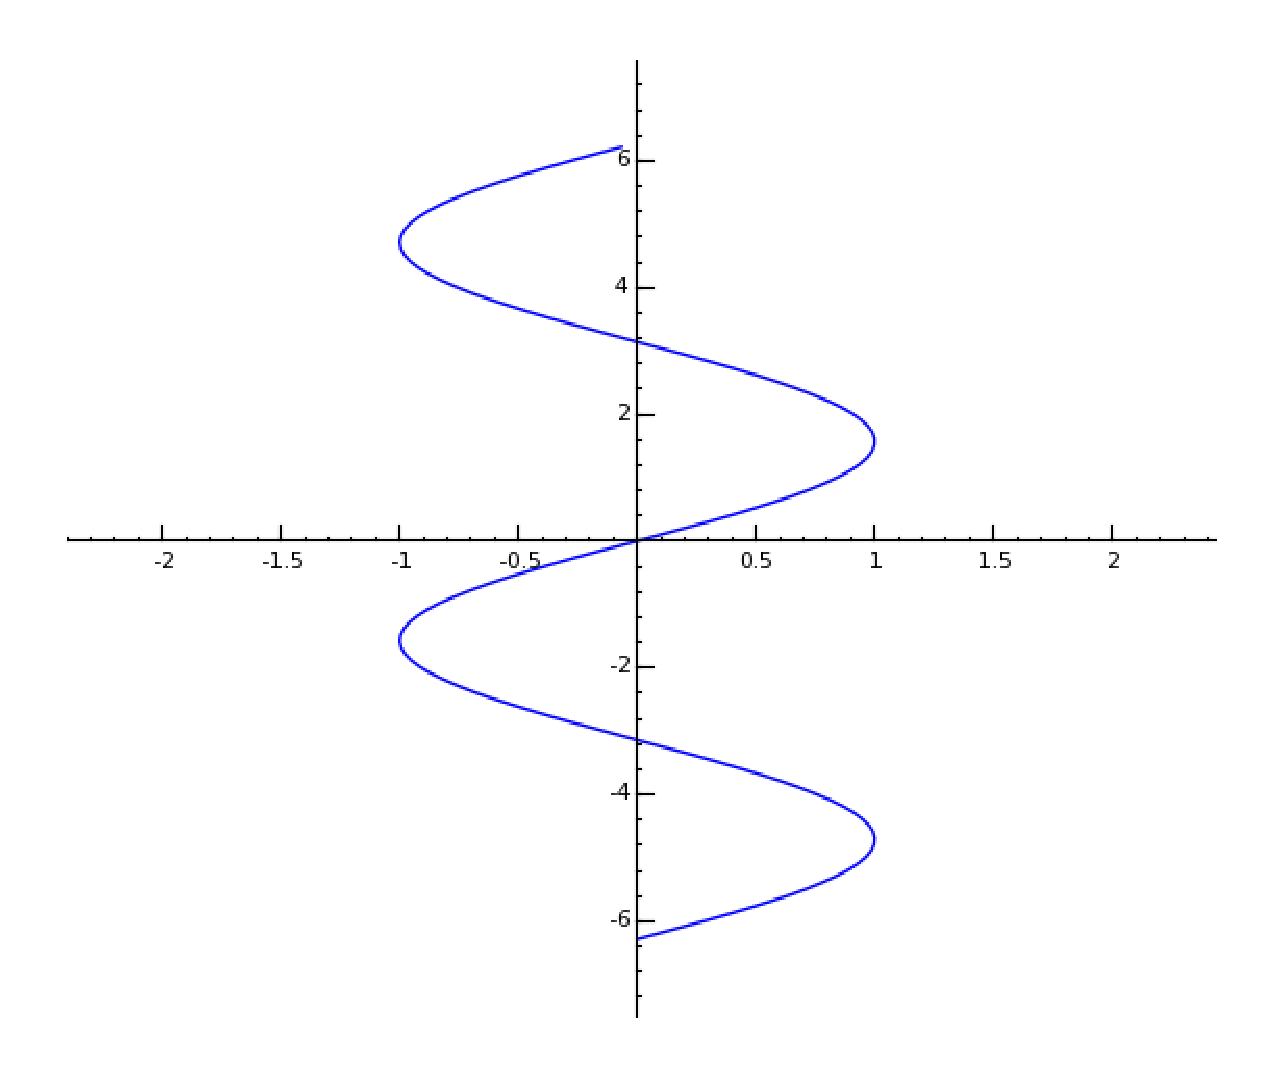
\includegraphics[height=6cm,width=7cm]{arcsin2.eps}
\end{center}
\end{minipage}
\caption{The inverse sine $\sin^{-1}\ x$ using \sage.}
\label{fig:arcsin2}
\end{figure}
%sage: v = [(sin(x),x) for x in srange(-2*float(pi),2*float(pi),0.1) if x]
%sage: show(line(v), xmin=-2, xmax=2)


\begin{figure}[h!]
%\begin{tabular}{cc}
\begin{minipage}{\textwidth}
\begin{center}
%\vspace{1.0 cm}
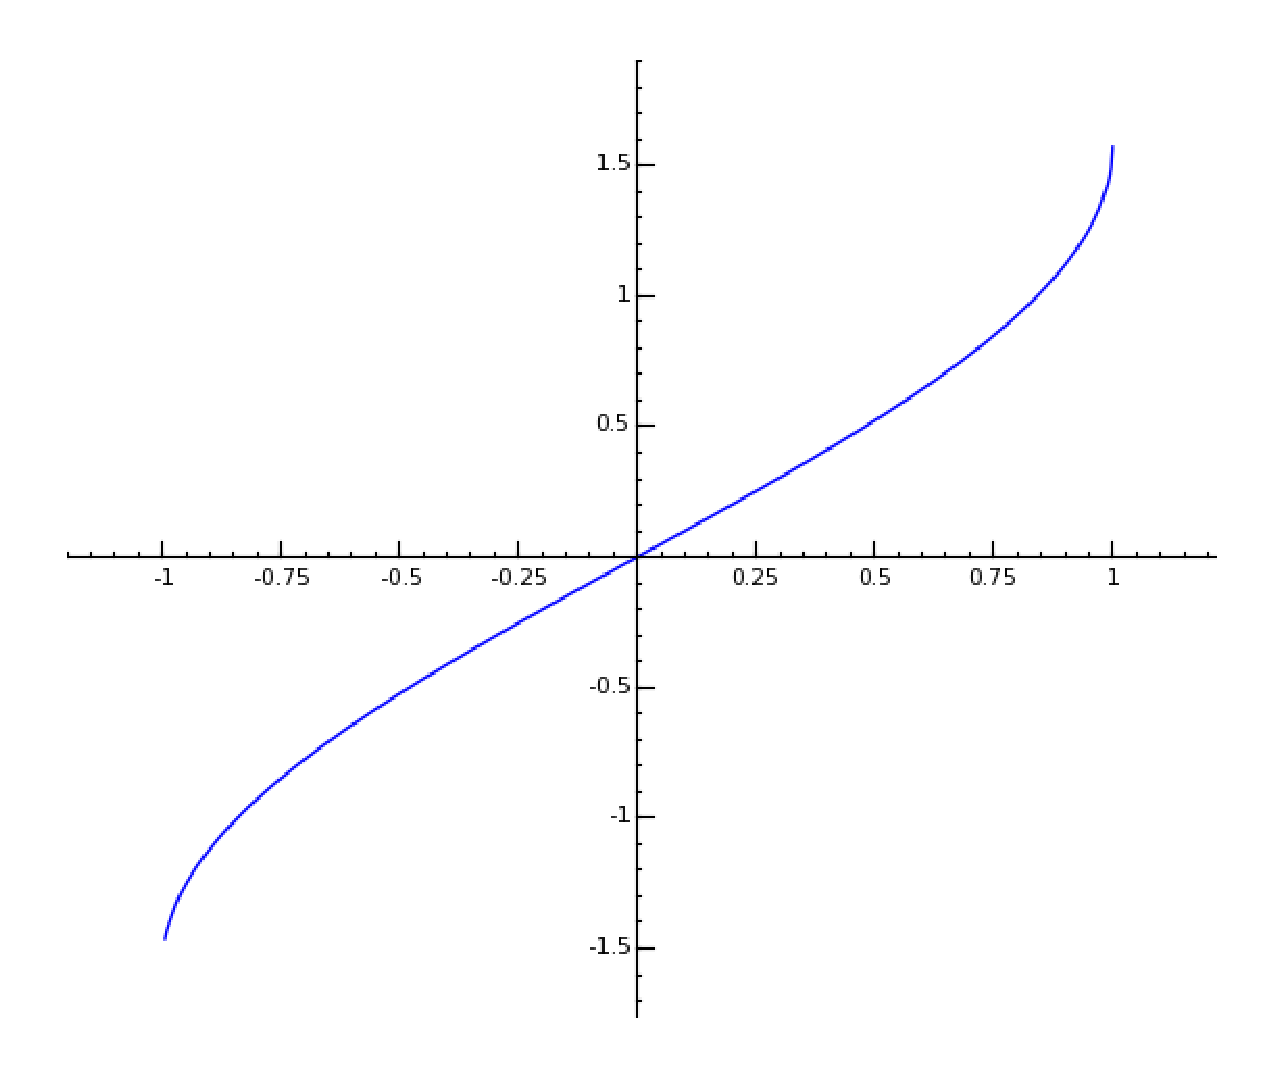
\includegraphics[height=3cm,width=3cm]{arcsin.eps}
\end{center}
\end{minipage}
\caption{A single branch of the function $f(x)=\arcsin(x)$.}
\label{fig:arcsin}
\end{figure}
%sage: show(plot(asin, -1,1))

\noindent
represents only a piece of the multi-valued inverse function of $\sin(x)$,
represented by taking the graph of $\sin(x)$ and flipping it about the 
$45^o$ line.
%when $v = OM$, $y = MP_1$, $MP_2$, $MP_3$, \dots, $MQ_1 MQ_2$, \dots.
In the above discussion, in order to make the function single-valued; 
only values of $y$ between $-\frac{\pi}{2}$ and $\frac{\pi}{2}$ inclusive %(points on arc QOP) 
are considered; that is, the arc of smallest numerical value whose sine is $v$. 

Differentiating $v$ with respect to $y$ by XI, $\frac{dv}{dy} 	= \cos\ y$;
therefore $\frac{dy}{dv} = \frac{1}{\cos y}$, by (\ref{eqn:C-43}). %, p. 46 [§ 43]
But since $v$ is a function of $x$, this may be substituted in
$\frac{dy}{dx} 	= \frac{dy}{dv} \cdot \frac{dv}{dx}$ (see (\ref{eqn:A-42})),%, p. 45 [§ 42]
giving 	

\[
\frac{dy}{dx} 	= \frac{1}{\cos y} \cdot \frac{dv}{dx} 	= \frac{1}{\sqrt{1 - v^2}} \frac{dv}{dx},
\]
(since $\cos y = \sqrt{1 - \sin^2 y} = \sqrt{1 - v^2}$), the positive sign 
of the radical being taken, since $\cos y$ is positive for all values of 
$y$ between $-\frac{\pi}{2}$ and $\frac{\pi}{2}$ inclusive). Therefore,
\[
\frac{d}{dx}(\arcsin\, v) 	= \frac{\frac{dv}{dx}}{\sqrt{1 - v^2}}
\]
(equation (XVIII) in \S \ref{sec:33}  above).

%56. 
\section{Differentiation of $\arccos v$}

Let\footnote{This function is defined only for values of $v$ between $-1$ and $+1$ inclusive, 
and is many-valued. %In the figure (the locus of y = arccosv), when v=OM, y=MP_1, MP_2, \cdots, MQ_1 MQ_2, \cdots.
In order to make the function single-valued, only values of $y$ between $0$ and $\pi$ 
inclusive are considered; that is, $y$ the smallest positive arc whose cosine is $v$. 
%Hence we confine ourselves to arc QP of the graph.
}
$ y 	= \arccos\ v$; then $y 	= \cos\ y$.


\begin{figure}[h!]
%\begin{tabular}{cc}
\begin{minipage}{\textwidth}
\begin{center}
%\vspace{1.0 cm}
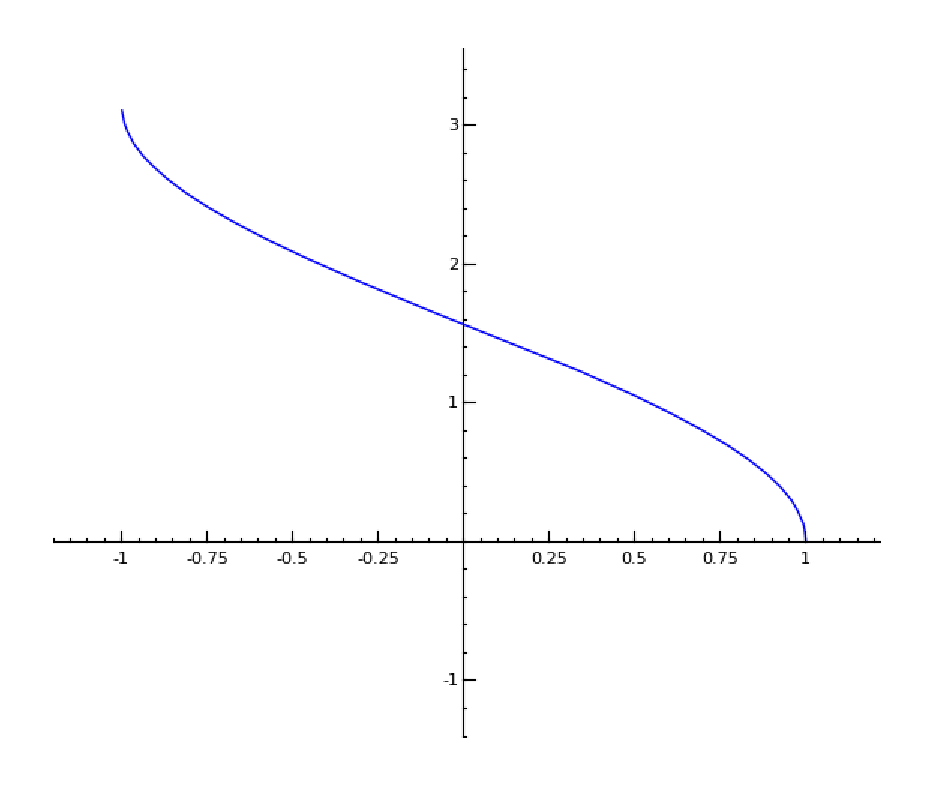
\includegraphics[height=3cm,width=3cm]{arccos2.eps}
\end{center}
\end{minipage}
\caption{A single branch of the function $f(x)=\arccos(x)$.}
\label{fig:arccos2}
\end{figure}
%sage: show(plot(acos, -1,1))

Differentiating with respect to $y$ by XII,
$  	\frac{dv}{dy} 	= -\sin\ y$,
therefore, $\frac{dy}{dv} = -\frac{1}{\sin y}$, by (\ref{eqn:C-43}). %, p. 46 [§ 43]
But since $v$ is a function of $x$, this may be substituted in the formula
$\frac{dy}{dx} 	= \frac{dy}{dv} \cdot \frac{dv}{dx}$, by (\ref{eqn:A-42}), %p. 45 [§ 42]
giving 	

\[
\frac{dy}{dx} 	= -\frac{1}{\sin y} \cdot \frac{dv}{dx}
  	= - \frac{1}{\sqrt{1 - v^2}} \frac{dv}{dx}
\]
($\sin y = \sqrt{1 - \cos^2 y} = \sqrt{1 - v^2}$, the plus sign of the radical 
being taken, since $\sin\, y$ is positive for all values of 
$y$ between $0$ and 
$\pi$ inclusive). 
Therefore,
\[
%XIX 	∴ 
\frac{d}{dx}(\arccos\, v) 	= -\frac{\frac{dv}{dx}}{\sqrt{1 - v^2}}.
\]
(equation (XIX) in \S \ref{sec:33}  above).


Here's how to use \sage to compute an example of this rule:

\vskip .2in

\begin{Verbatim}[fontsize=\scriptsize,fontfamily=courier,fontshape=tt,frame=single,label=\sage]

sage: t = var("t")
sage: x = var("x")
sage: solve(x == cos(t),t)
[t == acos(x)]
sage: f = solve(x == cos(t),t)[0].rhs()
sage: f
acos(x)
sage: diff(f,x)
-1/sqrt(1 - x^2)

\end{Verbatim}

\vskip .1in
\noindent
This (1) computes $\arccos$ directly as the inverse function of $\cos$
(\sage can use the notation ${\rm acos}$ in addition to $\arccos$), (2) computes
its derivative. 

\begin{figure}[h!]
%\begin{tabular}{cc}
\begin{minipage}{\textwidth}
\begin{center}
%\vspace{1.0 cm}
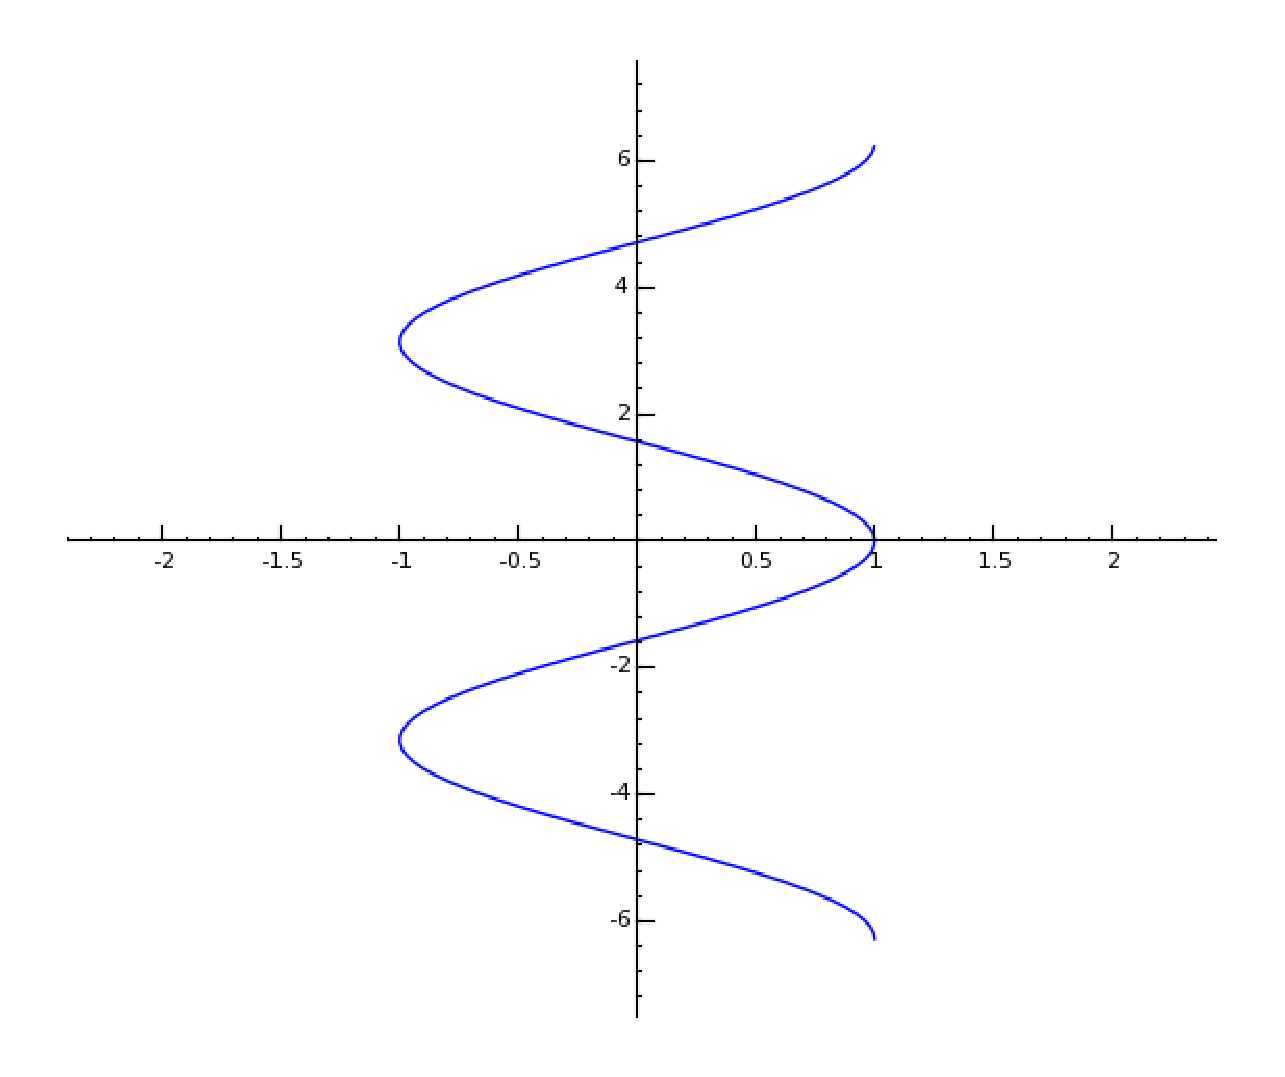
\includegraphics[height=6cm,width=7cm]{arccos.eps}
\end{center}
\end{minipage}
\caption{The inverse cosine $\cos^{-1}\ x$ using \sage.}
\label{fig:arccos}
\end{figure}
%sage: v = [(cos(x),x) for x in srange(-2*float(pi),2*float(pi),0.1) if x]
%sage: show(line(v), xmin=-2, xmax=2)



%57. 
\section{Differentiation of $\arctan\, v$}

Let\footnote{This function is defined for all values of $v$, and is 
many-valued. %, as is clearly shown by its graph. 
In order to make it single-valued, only values of $y$ between 
$-\frac{\pi}{2}$ and $\frac{\pi}{2}$ are considered; that is, the 
arc of smallest numerical value whose tangent is v.}% (branch AOE).}
$y 	=\ \arctan v$; then $y 	=\ \tan y$.


\begin{figure}[h!]
%\begin{tabular}{cc}
\begin{minipage}{\textwidth}
\begin{center}
%\vspace{1.0 cm}
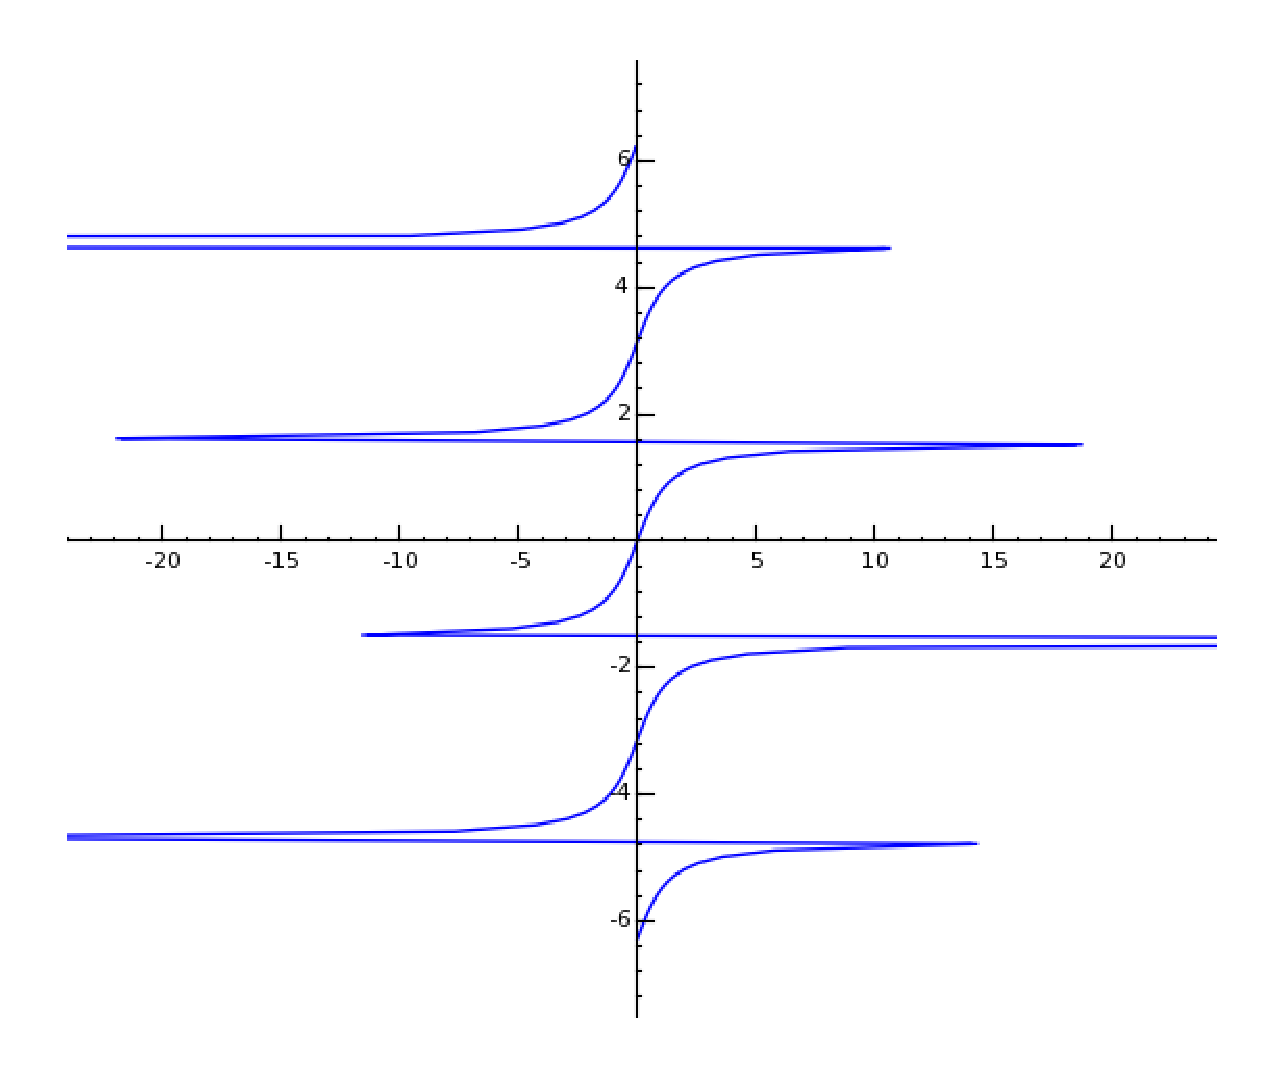
\includegraphics[height=6cm,width=7cm]{arctan2.eps}
\end{center}
\end{minipage}
\caption{The inverse tangent $\tan^{-1}\ x$ using \sage.}
\label{fig:arctan2}
\end{figure}
%sage: v = [(tan(x),x) for x in srange(-2*float(pi),2*float(pi),0.1) if x]
%sage: show(line(v), xmin=-20, xmax=20)

\begin{figure}[h!]
%\begin{tabular}{cc}
\begin{minipage}{\textwidth}
\begin{center}
%\vspace{1.0 cm}
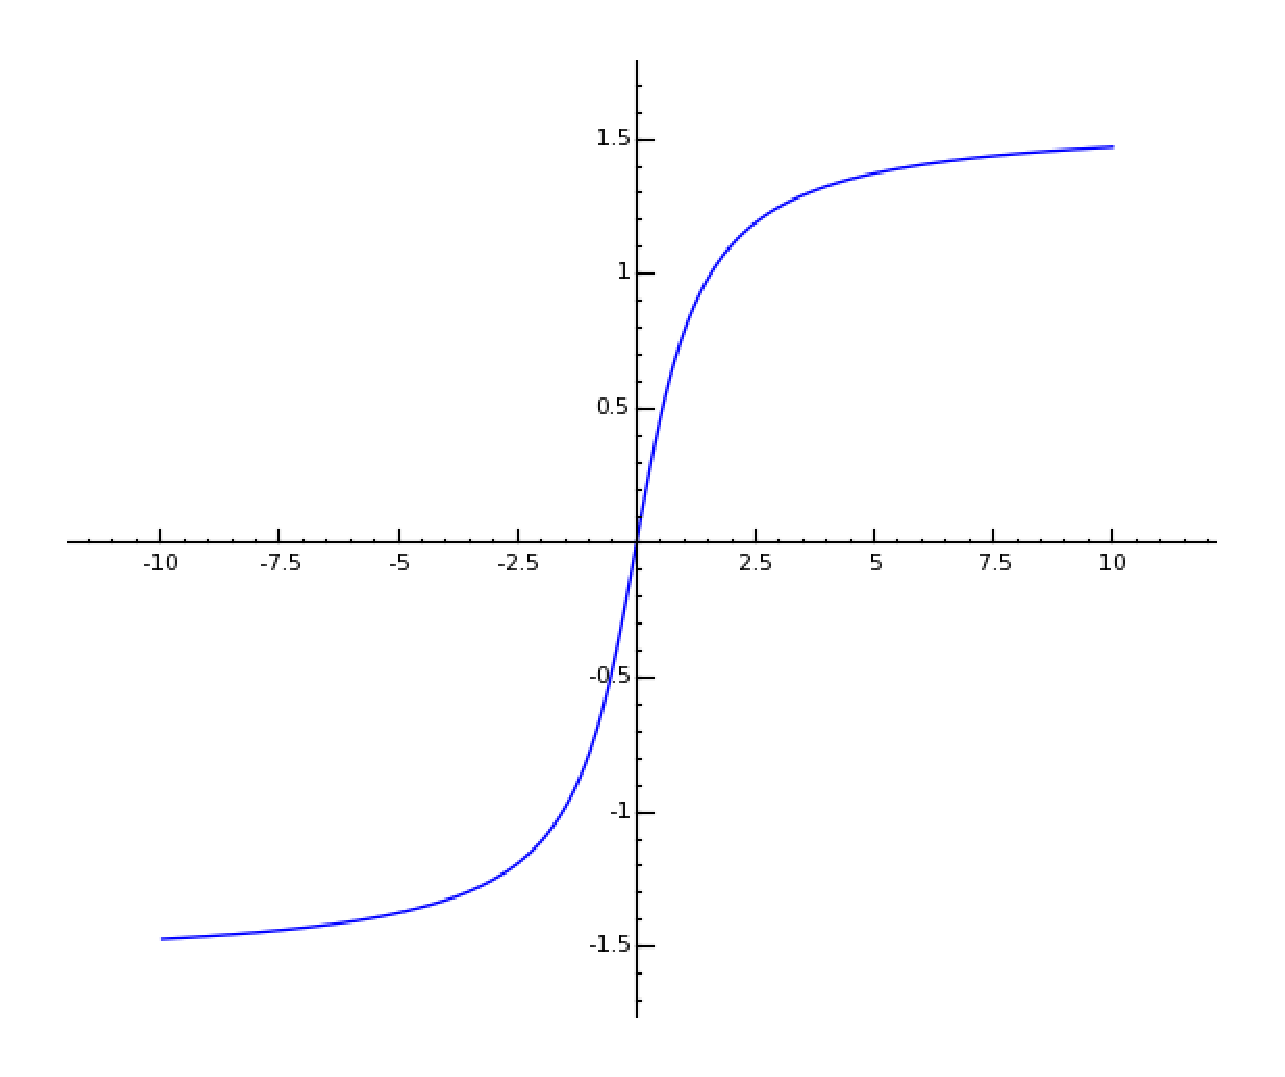
\includegraphics[height=5cm,width=8cm]{arctan.eps}
\end{center}
\end{minipage}
\caption{The standard branch of $\arctan\ x$ using \sage.}
\label{fig:arctan}
\end{figure}
%sage: show(plot(atan, -10,10))

Differentiating with respect to $y$ by (XIV),
\[
  	\frac{dv}{dy} 	=\ \sec^2 y;
\]
therefore $\frac{dy}{dv} 	= \frac{1}{\sec^2 y}$, by (\ref{eqn:C-43}). %, p. 46 [§ 43]
But since $v$ is a function of $x$, this may be substituted in the formula
$\frac{dy}{dx} 	= \frac{dy}{dv} \cdot \frac{dv}{dx}$, by (\ref{eqn:A-42}),% p. 45 [§ 42]
giving 	

\[
\frac{dy}{dx} 	= \frac{1}{\sec^2 y} \cdot \frac{dv}{dx}
  	= \frac{1}{1 + v^2} \frac{dv}{dx},
\]
(since $\sec^2y = 1 + \tan^2y = 1 + v^2$). Therefore
\[
%XX 	∴ 
\frac{d}{dx} (\arctan\, v) 	= \frac{\frac{dv}{dx}}{1 + v^2}
\]
(equation (XX) in \S \ref{sec:33}  above).



%58. 
\section{Differentiation of $\arccot u$}

Let $y 	= \arccot\ v$; then $y 	= \cot\ y$.
This function is defined for all values of $v$, and is many-valued.%, as is seen from its graph (Fig. a). 
In order to make it single-valued, only values of $y$ between $0$ and $\pi$ are considered; 
that is, the smallest positive arc whose cotangent is $v$. %Hence we confine ourselves to branch AB

Following the method of the last section, we get

\[
%XXI 
\frac{d}{dx}(\arccot\, v) = -\frac{\frac{dv}{dx}}{1 + v^2}
\]
(equation (XXI) in \S \ref{sec:33}  above).

\vskip .2in

\begin{Verbatim}[fontsize=\scriptsize,fontfamily=courier,fontshape=tt,frame=single,label=\sage]

sage: t = var('t')
sage: f = function('f', t)
sage: acot(f(t)).diff(t)
-diff(f(t), t, 1)/(f(t)^2 + 1)
sage: arccot(f(t)).diff(t)
-diff(f(t), t, 1)/(f(t)^2 + 1)
sage: f = lambda x: x^7
sage: arccot(f(t)).diff(t)
-7*t^6/(t^14 + 1)

\end{Verbatim}

%59. 
\section{Differentiation of $\arcsec u$}

Let
 $y 	=\ \arcsec v$; then $v 	=\ \sec y$.
This function is defined for all values of $v$ except those lying between $-1$ and $+1$, 
and is seen to be many-valued. To make the function single-valued, $y$ is taken as 
the arc of smallest numerical value whose secant is $v$. This means that if $v$ is positive, 
we confine ourselves to points on arc $AB$ (Figure \ref{fig:arcsec3}), $y$ taking on 
values between $0$ and $\frac{\pi}{2}$ ($0$ may be included); and if $v$ is negative, 
we confine ourselves to points on arc $DC$, $y$ taking on values between $-\pi$ and 
$-\frac{\pi}{2}$ ($-\pi$ may be included).

%\begin{figure}[h!]
%\begin{tabular}{cc}
%\begin{minipage}{\textwidth}
%\begin{center}
%\vspace{1.0 cm}
%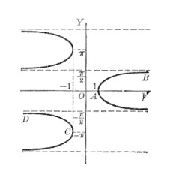
\includegraphics[height=4cm,width=3cm]{arcsec.eps}
%\end{center}
%\end{minipage}
%\caption{The inverse secant function $\arcsec x$ (scan of Granville's original graphic).}
%\label{fig:arcsec}
%\end{figure}


\begin{figure}[h!]
%\begin{tabular}{cc}
\begin{minipage}{\textwidth}
\begin{center}
%\vspace{1.0 cm}
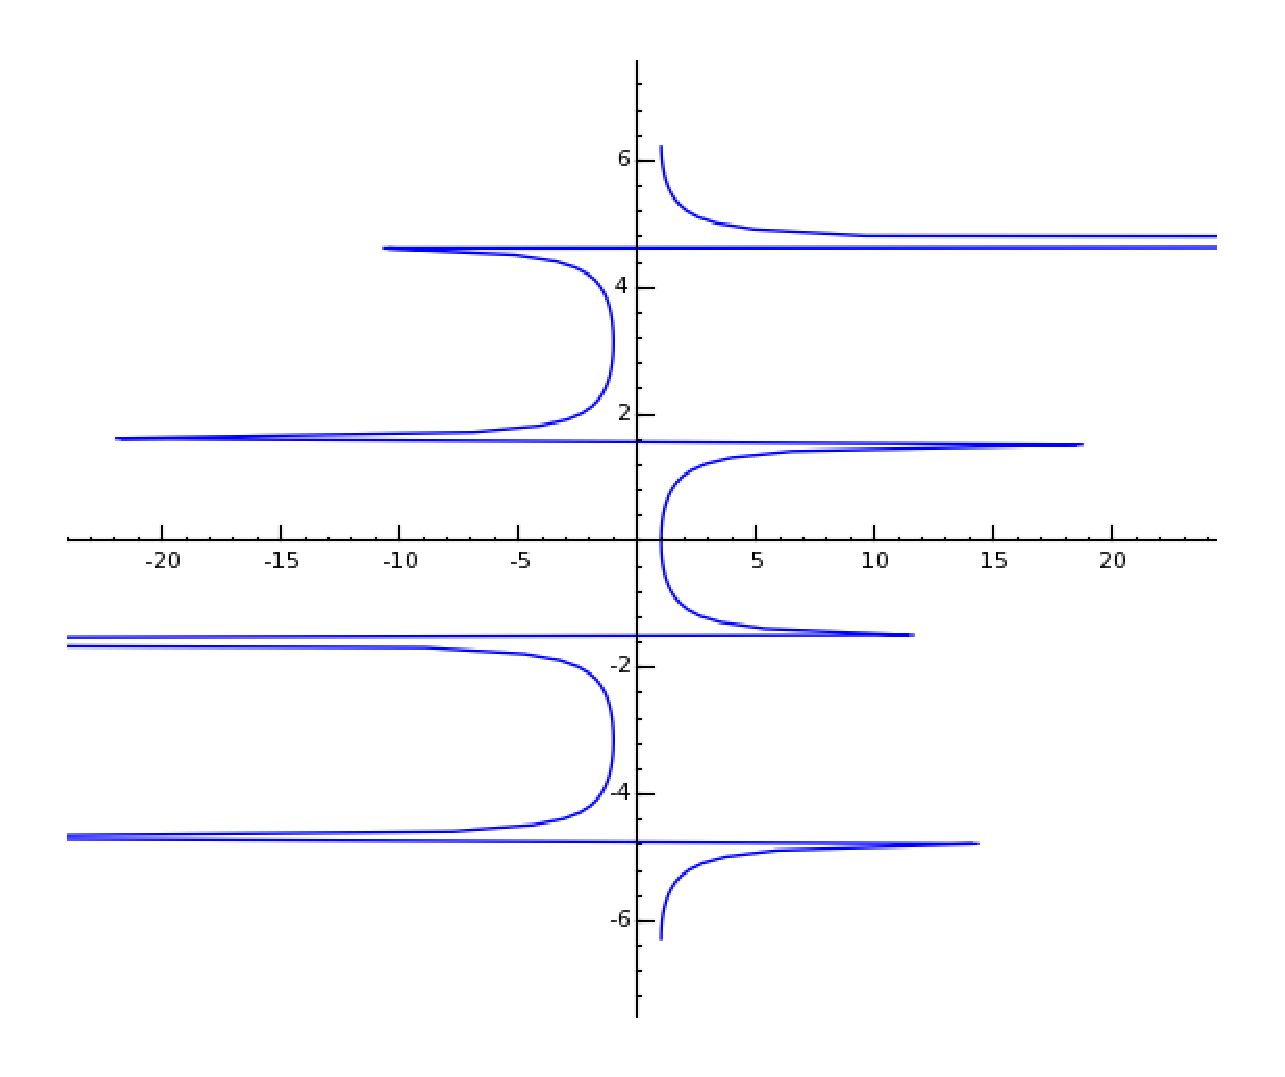
\includegraphics[height=6cm,width=7cm]{arcsec3.eps}
\end{center}
\end{minipage}
\caption{The inverse secant $\sec^{-1}\ x$ using \sage.}
\label{fig:arcsec3}
\end{figure}
%sage: v = [(sec(x),x) for x in srange(-2*float(pi),2*float(pi),0.1) if x]
%sage: show(line(v), xmin=-20, xmax=20)

\begin{figure}[h!]
%\begin{tabular}{cc}
\begin{minipage}{\textwidth}
\begin{center}
%\vspace{1.0 cm}
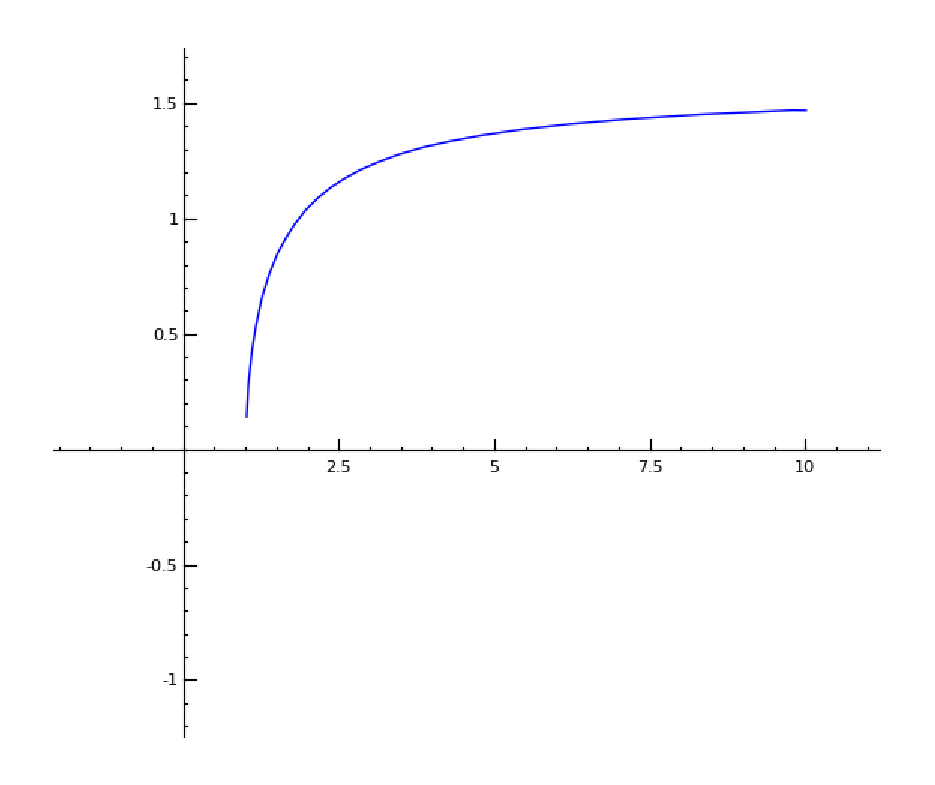
\includegraphics[height=5cm,width=8cm]{arcsec2.eps}
\end{center}
\end{minipage}
\caption{The standard branch of $\arcsec\ x$ using \sage.}
\label{fig:arcsec2}
\end{figure}
%sage: show(plot(asec, 1,10))

Differentiating with respect to $y$ by IV,
$\frac{dv}{dy} 	=\ \sec y \tan y$;
therefore $\frac{dy}{dv} 	= \frac{1}{\sec y \tan y}$, by (\ref{eqn:C-43}). %, p. 46 [§ 43]
But since $v$ is a function of $x$, this may be substituted in the formula
$\frac{dy}{dx} 	= \frac{dy}{dv} \cdot \frac{dv}{dx}$, by (\ref{eqn:A-42}).%	(A), p. 45 [§ 42]
giving 	

\[
\frac{dy}{dx} 	= \frac{1}{\sec y \tan y} \frac{dv}{dx}
  	= \frac{1}{v \sqrt{v^2 - 1}} \frac{dv}{dx}
\]
(since $\sec y = v$, and $\tan y = \sqrt{\sec y - 1} = \sqrt{v^2 - 1}$, the plus sign 
of the radical being taken, since $\tan y$ is positive for an values of $y$ between 
$0$ and $\frac{\pi}{2}$ and between $-\pi$ and $-\frac{\pi}{2}$, including 
$0$ and $-\pi$). Therefore,

\[
%XXII 	∴ 
\frac{d}{dx} (\arcsec v) 	= \frac{\frac{dv}{dx}}{v \sqrt{v^2 - 1}}
\]
(equation (XXII) in \S \ref{sec:33}  above).

%60. 
\section{Differentiation of $\arccsc\, v$}

Let 

\[
y 	=\ \arccsc\, v; 
\]
then 

\[
v =\ \csc\, y.
\]
This function is defined for all values of $v$ except those lying between $-1$ and $+1$, 
and is seen to be many-valued. To make the function single-valued, $y$ is taken as the 
arc of smallest numerical value whose cosecant is $v$. This means that if $v$ is positive, 
we confine ourselves to points on the arc $AB$ (Figure \ref{fig:arccsc2}), $y$ taking 
on values between $0$ and $\frac{\pi}{2}$ ($\frac{\pi}{2}$ may be included); 
and if $v$ is negative, we confine ourselves to points on the arc $CD$, $y$ taking on 
values between $-\pi$ and $-\frac{\pi}{2}$ ($-\frac{\pi}{2}$ may be included). 

%\newpage
%
%\begin{figure}[h!]
%\begin{tabular}{cc}
%\begin{minipage}{\textwidth}
%\begin{center}
%\vspace{1.0 cm}
%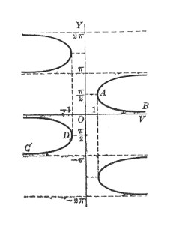
\includegraphics[height=4cm,width=3cm]{arccsc.eps}
%\end{center}
%\end{minipage}
%\caption{This is a scan of Granville's original graphic for $\arccsc\ x$.}
%\label{fig:arccsc}
%\end{figure}

\begin{figure}[h!]
%\begin{tabular}{cc}
\begin{minipage}{\textwidth}
\begin{center}
%\vspace{1.0 cm}
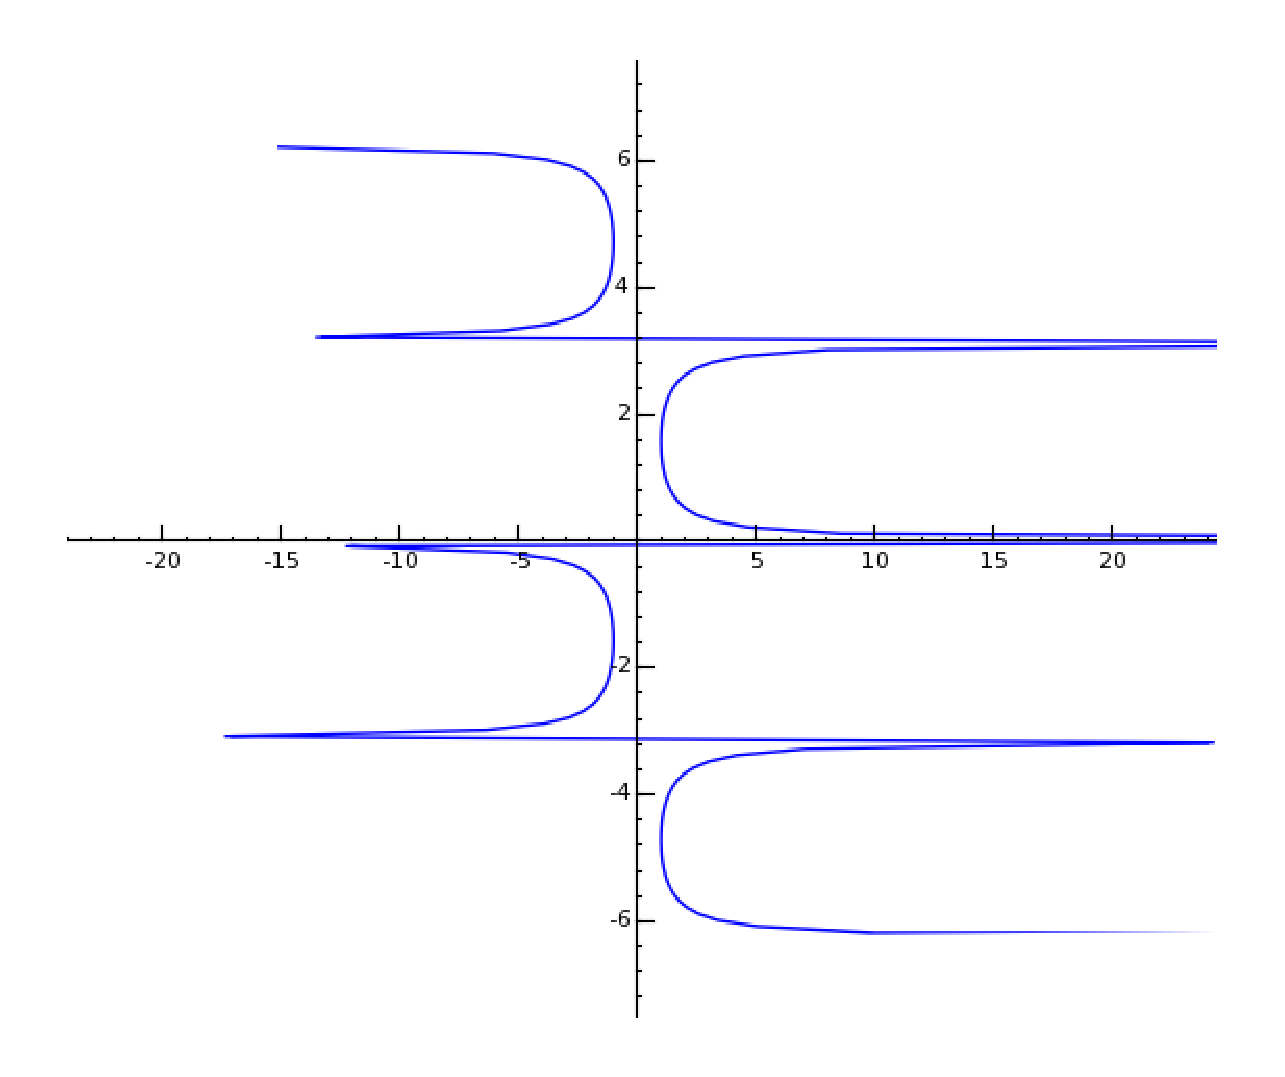
\includegraphics[height=6cm,width=7cm]{arccsc2.eps}
\end{center}
\end{minipage}
\caption{The inverse secant function $\arccsc\ x$ using \sage.}
\label{fig:arccsc2}
\end{figure}
%sage: v = [(csc(x),x) for x in srange(-2*float(pi),2*float(pi),0.1) if x]
%sage: show(line(v), xmin=-20, xmax=20)

\begin{figure}[h!]
%\begin{tabular}{cc}
\begin{minipage}{\textwidth}
\begin{center}
%\vspace{1.0 cm}
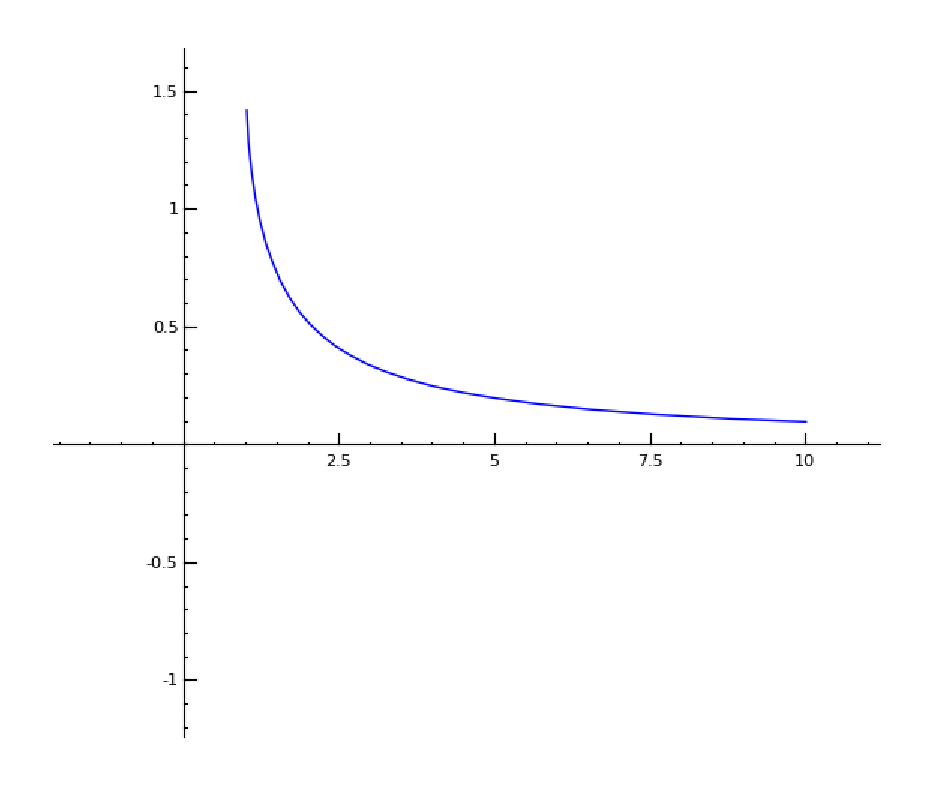
\includegraphics[height=5cm,width=8cm]{arccsc3.eps}
\end{center}
\end{minipage}
\caption{The standard branch of $\arccsc\ x$ using \sage.}
\label{fig:arccsc3}
\end{figure}

Differentiating with respect to $y$ by XVI and following the method of 
the last section, we get

\[
%XXIII 	
\frac{d}{dx}(\arccsc v) 	= -\frac{\frac{dv}{dx}}{v\sqrt{v^2 - 1}}
\]
(equation (XXIII) in \S \ref{sec:33}  above).


%61. 
\section{Differentiation of $\arcvers\, v$}

Let\footnote{Defined only for values of $v$ between $0$ and $2$ inclusive, and is 
many-valued. To make the function continuous, $y$ is taken as the smallest positive 
arc whose versed sine is $v$; that is, $y$ lies between $0$ and $\pi$ inclusive. 
%Hence we confine ourselves to arc OP of the graph (Fig. a).
}
$y 	= \arcvers\, v$; then $v = \vers\, y$.
Differentiating with respect to $y$ by XVII,
\[
  	\frac{dv}{dy} 	=\ \sin y;
\]
therefore $\frac{dy}{dv} 	= \frac{1}{\sin y}$, by (\ref{eqn:C-43}). %, p. 46 [§ 43]
But since $v$ is a function of $x$, this may be substituted in the formula
$\frac{dy}{dx} 	= \frac{dy}{dv} \cdot \frac{dv}{dx}$, by (\ref{eqn:A-42}).% 	(A), p. 45 [§ 42]
giving 	

\[
\frac{dy}{dx} 	= \frac{1}{\sin y} \cdot \frac{dv}{dx}
  	= \frac{1}{\sqrt{2v - v^2}} \frac{dv}{dx}
\]
(since $\sin y = \sqrt{1 - \cos^2 y} = \sqrt{1 - (1 - \vers\, y)^2} 
= \sqrt{2v - v^2}$, the plus sign of the radical being taken, since $\sin\, y$ 
is positive for all values of $y$ between $0$ and $\pi$ inclusive).
Therefore,
\[
%XXIV 	∴ 
\frac{d}{dx} (\operatorname{arcvers}\, v) 	= \frac{\frac{dv}{dx}}{\sqrt{2v - v^2}}
\]
(equation (XXIV) in \S \ref{sec:33}  above).


\section{Example}

Differentiate the following:

\begin{enumerate}
\item
%1. 
$y = \arctan (ax^2)$.

Solution. By XX ($v = ax^2$)

\[
\frac{dy}{dx} 	= \frac{\frac{d}{dx} (ax^2)}{1 + (ax^2)^2} 
  	= \frac{2ax}{1 + a^2x^4}.
\]

\item
%2
$y = \arcsin(3x - 4x^3)$.

Solution. By XVIII ($v = 3x - 4x^3$),

\[	
\frac{dy}{dx} =	\frac{\frac{d}{dx}(3x - 4x^3)}{\sqrt{1 - (3x - 4x^3)^2}}
=\frac{3 - 12x^2}{\sqrt{1 - 9x^2 + 24x^4 - 16x^6}} = \frac{3}{\sqrt{1 - x^2}}.
\]

\item
%3
$y=\arcsec\, \frac{x^2 + 1}{x^2 - 1}$.

Solution. By XXII ($v =  \frac{x^2 + 1}{x^2 - 1} $),	

\[
\frac{dy}{dx} 	
= \frac{\frac{d}{dx} \left ( \frac{x^2 + 1}{x^2 - 1} \right )}{\frac{x^2 + 1}{x^2 - 1} \sqrt{\left ( \frac{x^2 + 1}{x^2 - 1} \right )^2 - 1}} 	
= \frac{\frac{(x^2 - 1)2x - (x^2 + 1)2x}{(x^2 - 1)^2}}{\frac{x^2 + 1}{x^2 - 1} \cdot \frac{2x}{x^2 - 1}} 
= -\frac{2}{x^2 + 1}.
\]

\item
%4
$\frac{d}{dx} \arcsin \frac{x}{a} = \frac{1}{\sqrt{a^2 - x^2}}$

\item
%5
$\frac{d}{dx} \arccot (x^2 - 5) = \frac{-2x}{1 + (x^2 - 5)^2}$

\item
%6
$\frac{d}{dx} \arctan \frac{2x}{1 - x^2} = \frac{2}{1 + x^2}$

\item
%7
$\frac{d}{dx} \arccsc \frac{1}{2x^2 - 1} = \frac{2}{\sqrt{1 - x^2}}$

\item
%8
$\frac{d}{dx} \operatorname{arcvers}\, 2x^2 = \frac{2}{\sqrt{1 - x^2}}$

\item
%9
$\frac{d}{dx} \arctan \sqrt{1 - x} = -\frac{1}{2 \sqrt{1 - x} (2 - x)}$

\item
%10
$\frac{d}{dx} \arccsc \frac{3}{2x} = \frac{2}{9 - 4x^2}$

\item
%11
$\frac{d}{dx} \operatorname{arcvers}\, \frac{2x^2}{1 + x^2} = \frac{2}{1 + x^2}$

\item
%12
$\frac{d}{dx} \arctan \frac{x}{a} = \frac{a}{a^2 + x^2}$

\item
%13
$\frac{d}{dx} \arcsin \frac{x + 1}{\sqrt{2}} = \frac{1}{\sqrt{1 - 2x - x^2}}$

\item
%14
$f(x) = x\sqrt{a^2 - x^2} + a^2 \arcsin \frac{x}{a}$\qquad\qquad\qquad\qquad\qquad Ans: 
$ f'(x) =\ 2\sqrt{a^2 - x^2}$

\item
%15
$f(x) = \sqrt{a^2 - x^2} + a \arcsin \frac{x}{a}$\qquad\qquad\qquad\qquad\qquad Ans: 
$f'(x) 	= \left ( \frac{a - x}{a + x} \right )^{\frac{1}{2}}$

\item
%16
$x = r \arcvers\, \frac{y}{r} - \sqrt{2ry - y^2}$\qquad\qquad\qquad\qquad\qquad\qquad Ans: 
$\frac{dx}{dy} 	= \frac{y}{\sqrt{2ry - y^2}}$

\item
%17
$\theta = \arcsin (3r - 1)$\qquad\qquad\qquad\qquad\qquad\qquad Ans:  	
$\frac{d\theta}{dr} 	= \frac{3}{\sqrt{6r - 9r^2}}$

\item
%18
$\phi = \arctan \frac{r + a}{1 - ar}$\qquad\qquad\qquad\qquad\qquad\qquad Ans: 
$\frac{d\phi}{dr} 	= \frac{1}{1 + r^2}$

\item
%19
$s = \arcsec \frac{1}{\sqrt{1 - t^2}}$\qquad\qquad\qquad\qquad\qquad\qquad Ans:  
$\frac{ds}{dt} =	\frac{1}{\sqrt{1 - t^2}}$

\item
%20
$\frac{d}{dx} ( x \arcsin\, x) = \arcsin\, x + \frac{x}{\sqrt{1 - x^2}}$

\item
%21
$\frac{d}{d\theta} (\tan \theta \arctan\, \theta) 
= \sec^2 \theta \arctan\, \theta \frac{\tan \theta}{1 + \theta^2}$

\item
%22
$\frac{d}{dt}[\log (\arccos\, t)] = -\frac{1}{\arccos t \sqrt{1 - t^2}}$

\item
%23
$f(y) = \arccos (\log\, y)$ \qquad\qquad\qquad\qquad\qquad\qquad Ans:  	
$f'(y) 	= -\frac{1}{y\sqrt{1 - (\log y)^2}}$

\item
%24
$f(\theta) = \arcsin \sqrt{\sin \theta}$\qquad\qquad\qquad\qquad\qquad\qquad Ans: 
$f'(\theta) 	= \frac{1}{2} \sqrt{1 + \csc \theta}$

\item
%25
$f(\phi) = \arctan \sqrt{\frac{1 - \cos \phi}{1 + \cos \phi}}$\qquad\qquad\qquad\qquad\qquad\qquad Ans:  
$f'(\phi) 	= \frac{1}{2}$

\item
%26
$p = e^{\arctan\, q}$ \qquad\qquad\qquad\qquad\qquad\qquad Ans:  	
$\frac{dp}{dq} 	= \frac{e^{\arctan\, q}}{1 + q^2}$

\item
%27
$u = \arctan \frac{e^v - e^{-v}}{2}$\qquad\qquad\qquad\qquad\qquad\qquad Ans:  	
$\frac{du}{dv} 	= \frac{2}{e^v + e^{-v}}$

\item
%28
$s = \arccos \frac{e^t - e^{-t}}{e^t + e^{-t}}$\qquad\qquad\qquad\qquad\qquad\qquad Ans:  
$\frac{ds}{dt} 	= -\frac{2}{e^v + e^{-v}}$

\item
%29
$y = x^{\arcsin x}$\qquad\qquad\qquad\qquad\qquad\qquad Ans:  	
$y' = x^{\arcsin x} \left ( \frac{\arcsin x}{x} + \frac{\log x}{\sqrt{1 - x^2}} \right )$

\item
%30
$y = e^{x^x} \arctan\, x$\qquad\qquad\qquad\qquad\qquad\qquad Ans:  	
$y' 	= e^{x^x} \left [ \frac{1}{1 + x^2} + x^x \arctan x (1 + \log x) \right ]$

\item
%31
$y = \arcsin( \sin x )$\qquad\qquad\qquad\qquad\qquad\qquad Ans:  	
$y' = 1$

\item
%32
$y = \arctan \frac{4 \sin x}{3 + 5 \cos x}$\qquad\qquad\qquad\qquad\qquad\qquad Ans:  
$y' 	= \frac{4}{5 + 3 \cos x}$

\item
%33
$y = \arccot \frac{a}{x} + \log \sqrt{\frac{x - a}{x + a}}$\qquad\qquad\qquad\qquad\qquad\qquad Ans:  	
$y' 	= \frac{2ax^2}{x^4 - a^4}$

\item
%34
$y = \log \left ( \frac{1 + x}{1 - x} \right )^{\frac{1}{4}} - \frac{1}{2} \arctan\, x$\qquad\qquad\qquad\qquad\qquad\qquad Ans:  
$y' 	= \frac{x^2}{1 - x^4}$

\item
%35
$y = \sqrt{1 - x^2} \arcsin\, x - x$\qquad\qquad\qquad\qquad\qquad\qquad Ans:  	
$y' 	= - \frac{x \arcsin\, x}{\sqrt{1 - x^2}}$

\item
%36
%Differentiate the following functions:
Compute the following derivatives:

\[
\begin{array}{lll}
(a)\ \  \frac{d}{dx} \arcsin 2x^2  &   	(f)\ \  \frac{d}{dt} t^3 \arcsin \frac{t}{3}  &   	(k)\ \  \frac{d}{dy} \arcsin \sqrt{1 - y^2}\\
 & & \\
(b)\ \  \frac{d}{dx} \arctan a^2x  &   	(g)\ \  \frac{d}{dt} e^{\arctan at}  &   	(l)\ \  \frac{d}{dz} \arctan ( \log 3 az )\\
 & & \\
(c)\ \  \frac{d}{dx} \arcsec \frac{x}{a}  &   	(h)\ \  \frac{d}{d\phi} \tan \phi^2 \cdot \arctan \phi^{\frac{1}{2}}  &   	(m)\ \  \frac{d}{ds}(a^2 + s^2)\arcsec \frac{s}{2}\\
 & & \\
(d)\ \  \frac{d}{dx} x \arccos x  &   	(i)\ \  \frac{d}{d\theta} \arcsin a^{\theta}  &   	(n)\ \  \frac{d}{d\alpha} \arccot \frac{2\alpha}{3}\\
 & & \\
(e)\ \  \frac{d}{dx} x^2 \arccot ax  &   	(j)\ \  \frac{d}{d\theta} \arctan \sqrt{1 + \theta^2}  &   	(o)\ \  \frac{d}{dt} \sqrt{1 - t^2} \arcsin t
\end{array}
\]

\end{enumerate}

Formulas (\ref{eqn:A-42}) %, p. 45 [§ 42], 
for differentiating a function of a function, and (\ref{eqn:C-43}) %, p. 46 [§ 43], 
for differentiating inverse junctions, have been added to the list of 
formulas at the beginning of this chapter as XXV and XXVI respectively.

In the next eight examples, first find $\frac{dy}{dv}$ and $\frac{dv}{dx}$ by 
differentiation and then substitute the results in
$\frac{dy}{dx} 	= \frac{dy}{dv} \cdot \frac{dv}{dx}$ (by XXV)
to find $\frac{dy}{dx}$. (As was pointed out in \S \ref{sec:42}, %on p. 44 [§ 42], 
it might be possible to eliminate $v$ between the two given expressions so 
as to find $y$ directly as a function of $x$, but in most cases the above method is to be preferred.)

In general our results should be expressed explicitly in terms of the 
independent variable; that is, $\frac{dy}{dx}$ in terms of $x$, 
$\frac{dx}{dy}$ in terms of $y$, $\frac{d\phi}{d\theta}$ in terms of $\theta$, etc.

\begin{enumerate}
\addtocounter{enumi}{36}
\item
%37
$y = 2v^2 - 4$, $v = 3x^2 + 1$.

$\frac{dy}{dv} = 4v$; $\frac{dv}{dx} = 6x$; substituting in XXV,
$\frac{dy}{dx} = 4v \cdot 6x = 24x(3x^2 + 1)$.

\item
%38
$y = \tan 2v$, $v = \arctan(2x - 1)$.

$\frac{dy}{dv} = 2 \sec^2 2v$; $\frac{dv}{dx} = \frac{1}{2x^2 - 2x + 1}$; substituting in XXV,

\[
\frac{dy}{dx} = \frac{2 \sec^2 2v}{2x^2 - 2x + 1} 
= 2 \frac{\tan^2 2v + 1}{2x^2 - 2x + 1} 
= \frac{2x^2 - 2x + 1}{2(x - x^2)^2}
\]
(since $v = \arctan (2x - 1)$, $\tan v = 2x - 1$, $\tan 2v = \frac{2x - 1}{2x - 2x^2}$).

\item
%39
$y = 3 v^2 - 4v + 5, v = 2x^3 - 5$\qquad\qquad\qquad\qquad\qquad\qquad Ans:  
$\frac{dy}{dx} 	=\ 72x^5 - 204x^2$

\item
%40
$y = \frac{2v}{3v - 2}, v = \frac{x}{2x - 1}$\qquad\qquad\qquad\qquad\qquad\qquad Ans:  
$\frac{dy}{dx} 	= \frac{4}{(x - 2)^2}$

\item
%41
$y = \log(a^2 - v^2)$\qquad\qquad\qquad\qquad\qquad\qquad Ans:  
$\frac{dy}{dx} 	=\ -2 \tan x$

\item
%42
$y = \arctan (a + v), v = e^x$\qquad\qquad\qquad\qquad\qquad\qquad Ans: 
$\frac{dy}{dx} 	=\ \frac{e^x}{1 + (a + e^x)^2}$

\item
%43
$r = e^{2s} + e^s, s = \log(t - t^2)$\qquad\qquad\qquad\qquad\qquad\qquad Ans:  	
$\frac{dr}{dt} 	=\ 4t^3 - 6t^2 + 1$
\end{enumerate}

In the following examples first find $\frac{dx}{dy}$ by differentiation 
and then substitute in

\[
\frac{dy}{dx} 	=\ \frac{1}{\frac{dx}{dy}}\ \ \ \ {\rm	by\ XXVI}
\]
to find $\frac{dy}{dx}$.

\begin{enumerate}
\addtocounter{enumi}{43}
\item
%44
$x = y\sqrt{1 + y}$\qquad\qquad\qquad\qquad\qquad\qquad Ans:  	
$\frac{dy}{dx} 	=\ \frac{2\sqrt{1 + y}}{2 + 3y} = \frac{2x}{2y + 3y^2}$

\item
%45
$x = \sqrt{1 + \cos\, y}$\qquad\qquad\qquad\qquad\qquad\qquad Ans:  	
$\frac{dy}{dx} 	=\ -\frac{2 \sqrt{1 + \cos\, y}}{\sin\, y} = -\frac{2}{\sqrt{2 - x^2}}$

\item
%46
$x = \frac{y}{1 + \log\, y}$\qquad\qquad\qquad\qquad\qquad\qquad Ans:  	
$\frac{dy}{dx} 	=\ \frac{(1 + \log y)^2}{\log\, y}$

\item
%47
$x = a \log \frac{a + \sqrt{a^2 - y^2}}{y}$\qquad\qquad\qquad\qquad\qquad\qquad Ans:  
$\frac{dy}{dx} 	=\ -\frac{y \sqrt{a^2 - y^2}}{a^2}$

\item
%48
$x = r \arcvers\, \frac{y}{r} - \sqrt{2ry - y^2}$\qquad\qquad\qquad\qquad\qquad\qquad Ans:  
$\frac{dy}{dx} 	=\ \sqrt{\frac{2r - y}{y}}$

\item
%49
Show that the geometrical significance of XXVI is 
that the tangent makes complementary angles with the two coordinate axes.


\end{enumerate}

%62. 
\section{Implicit functions}

When a relation between $x$ and $y$ is given by means of an equation 
not solved for $y$, then $y$ is called an implicit function of $x$. 
For example, the equation

\[
    x^2 - 4y = 0
\]
defines $y$ as an implicit function of $x$. Evidently $x$ is also defined 
by means of this equation as an implicit function of $y$. Similarly,

\[
    x^2 + y^2 + z^2 - a^2 = 0
\]
defines anyone of the three variables as an implicit function of the other two.

It is sometimes possible to solve the equation defining an implicit 
function for one of the variables and thus change it into an explicit 
function. For instance, the above two implicit functions may be solved for $y$, 
giving $y 	= \frac{x^2}{4}$
and $ y 	= \pm \sqrt{a^2 - x^2 - z^2}$;
the first showing $y$ as an explicit function of $x$, and the second as 
an explicit function of $x$ and $z$. In a given case, however, 
such a solution may be either impossible or too complicated for convenient use.

The two implicit functions used in this %article 
section % new
for illustration may be respectively denoted by
$f(x,y) 	= 0$ and $F(x,y,z) 	= 0$.


%63. 
\section{Differentiation of implicit functions}
\label{sec:63}

When $y$ is defined as an implicit function of $x$ by means of an equation in the form

\begin{equation}
%  (A) 
f(x,y) = 0,
\label{eqn:A-63}
\end{equation}
it was explained in the last section how it might be inconvenient to solve 
for $y$ in terms of $x$; that is, to find $y$ as an explicit function of $x$ 
so that the formulas we have deduced in this chapter may be applied 
directly. Such, for instance, would be the case for the equation

\begin{equation}
%     (B) 
ax^6 + 2x^3y - y^7x - 10 = 0.
\label{eqn:B-63}
\end{equation}
We then follow the rule:

{\it Differentiate, regarding $y$ as a function of $x$, 
and put the result equal to zero
\footnote{%This process will be justified in \S \ref{sec:127} %§127. 
Only corresponding values of $x$ and $y$ which satisfy the given equation 
may be substituted in the derivative.}.}
That is,

\begin{equation}
%    (C) 
\frac{d}{dx} f(x, y) = 0.
\label{eqn:C-63}
\end{equation}
Let us apply this rule in finding $\frac{dy}{dx}$ from (\ref{eqn:B-63}):
by (\ref{eqn:C-63}),

\[
\frac{d}{dx}(ax^6 + 2x^3y - y^7x - 10) = 0,
\]
\[
\frac{d}{dx}(ax^6) + \frac{d}{dx}(2x^3y) - \frac{d}{dx}(y^7x) - \frac{d}{dx}(10) = 0;
\]
\[
6ax^5 + 2x^3 \frac{dy}{dx} + 6x^2y - y^7 - 7xy^6\frac{dy}{dx} = 0;
\]
\[
(2x^3 - 7xy^6)\frac{dy}{dx} = y^7 - 6ax^5 - 6x^2y;
\]
\[
\frac{dy}{dx} = \frac{y^7 - 6ax^5 - 6x^2y}{2x^3 - 7xy^6} .
\]
This is the final answer.

The student should observe that in general the result will contain both $x$ and $y$.

\section{Exercises}

Differentiate the following by the above rule:

\begin{enumerate}

\item
%1
$y^2 = 4px$\qquad\qquad\qquad\qquad\qquad\qquad Ans:  
$\frac{dy}{dx} 	=\ \frac{2p}{y}$

\item
%2
$x^2 + y^2 = r^2$\qquad\qquad\qquad\qquad\qquad\qquad Ans:  	
$\frac{dy}{dx} 	=\ -\frac{x}{y}$

\item
%3
$b^2x^2 + a^2y^2 = a^2b^2$\qquad\qquad\qquad\qquad\qquad\qquad Ans: 
$\frac{dy}{dx} 	=\ -\frac{b^2x}{a^2y}$

\item
%4
$y^3 - 3y + 2ax = 0$\qquad\qquad\qquad\qquad\qquad\qquad Ans:  
$\frac{dy}{dx} 	=\ \frac{2a}{3(1 - y^2)}$

\item
%5
$x^{\frac{1}{2}} + y^{\frac{1}{2}} = a^{\frac{1}{2}}$\qquad\qquad\qquad\qquad\qquad\qquad Ans:  
$\frac{dy}{dx} 	=\ -\sqrt{\frac{y}{x}}$

\item
%6
$x^{\frac{2}{3}} + y^{\frac{2}{3}} = a^{\frac{2}{3}}$\qquad\qquad\qquad\qquad\qquad\qquad Ans: 
$\frac{dy}{dx} 	=\ -\sqrt[3]{\frac{y}{x}}$

\item
%7
$\left ( \frac{x}{a} \right )^2 + \left ( \frac{y}{b} \right )^{\frac{2}{3}} = 1$\qquad\qquad\qquad\qquad\qquad\qquad Ans:  	
$\frac{dy}{dx} 	=\ -\frac{3b^{\frac{2}{3}}xy^{\frac{1}{3}}}{a^2}$

\item
%8
$y^2 - 2xy + b^2 = 0$\qquad\qquad\qquad\qquad\qquad\qquad Ans:  
$\frac{dy}{dx} 	=\ \frac{y}{y - x}$

\item
%9
$x^3 + y^3 - 3axy = 0$\qquad\qquad\qquad\qquad\qquad\qquad Ans: 
$\frac{dy}{dx} 	=\ \frac{ay - x^2}{y^2 - ax}$

\item
%10
$x^y = y^x$\qquad\qquad\qquad\qquad\qquad\qquad Ans:  
$\frac{dy}{dx} 	=\ \frac{y^2 - xy\log\, y}{x^2 - xy\log\, x}$

\item
%11
$\rho^2 = a^2 \cos 2\theta$\qquad\qquad\qquad\qquad\qquad\qquad Ans:  	
$\frac{d\rho}{d\theta} 	=\ -\frac{a^2 \sin 2\theta}{\rho}$

\item
%12
$\rho^2 \cos\, \theta = a^2 \sin\, 3\theta$\qquad\qquad\qquad\qquad\qquad\qquad Ans:  	
$\frac{d\rho}{d\theta} 	=\ \frac{3a^2 \cos\, 3\theta + \rho^2 \sin\, \theta}{2\rho \cos\, \theta}$

\item
%13
$\cos(uv) = cv$\qquad\qquad\qquad\qquad\qquad\qquad Ans:  	
$\frac{du}{dv} 	=\ \frac{c + u\sin(uv)}{-v\sin(uv)}$

\item
%14
$\theta = \cos(\theta + \phi)$\qquad\qquad\qquad\qquad\qquad\qquad Ans: 
$\frac{d\theta}{d\phi} 	=\ -\frac{\sin(\theta + \phi)}{1 + \sin(\theta + \phi)}$

\item
%15
Find $\frac{dy}{dx}$ from the following equations:

\[
\begin{array}{lll}
(a)\ \  x^2 = ay & 	(f)\ \  xy + y^2 + 4x = 0 &	(k)\ \  \tan\, x + y^3 = 0\\
(b)\ \  x^2 + 4y^2 = 16  & 	(g)\ \  yx^2 - y^3 = 5 & 	(l)\ \  \cos\, y + 3x^2 = 0\\
(c)\ \  b^2x^2 - a^2y^2 = a^2b^2  & (h)\ \  x^2 - 2x^3 = y^3 & 	(m)\ \  x\cot\, y + y = 0\\
(d)\ \  y^2 = x^3 + a  & 	(i)\ \  x^2y^3 + 4y = 0  & 	(n)\ \  y^2 = \log\, x\\
(e)\ \  x^2 - y^2 = 16  &  (j)\ \  y^2 = \sin\, 2x  & 	(o)\ \  e^{x^2} + 2y^3 = 0
\end{array}
\]

\item
%16
A race track has the form of the circle $x^2 + y^2 = 2500$. The 
$x$-axis and $y$-axis are east and north respectively, 
and the unit is $1$ rod\footnote{
%Added 2007:
The {\it rod} is a unit of length equal to $15.5$ feet (about $5$ meters).
\index{rod} % new
}. 
If a runner starts east at the extreme north point, in what direction will he be going

\begin{tabular}{ll}
(a) when $25\sqrt{2}$ rods east of OY? &{\small{	Ans. 	Southeast or southwest.}}\\
(b) when $25\sqrt{2}$ rods north of OX? &{\small{	  Ans. 	Southeast or northeast.}}\\
(c) when 30 rods west of OY? 	&  {\small{Ans. 	E. $36^o$ 52' 12'' N. or W. $36^o$ 52' 12'' N.}}\\
(d) when 40 rods south of OX? & \\
(e) when 10 rods east of OY? & \\
\end{tabular}

\item
%17
An automobile course is elliptic in form, the major axis being $6$ miles long 
and running east and west, while the minor axis is $2$ miles long. If a 
car starts north at the extreme east point of the course, in what direction will the car be going

(a) when $2$ miles west of the starting point?

(b) when $1/2$ mile north of the starting point?
\end{enumerate}

\section{Miscellaneous Exercises}

Differentiate the following functions:

\begin{enumerate}

\item
%1
$\arcsin \sqrt{1 - 4x^2}$
	\qquad\qquad\qquad\qquad\qquad\qquad Ans:  
$\frac{-2}{\sqrt{1 - 4x^2}}$

\item
%2
$xe^{x^2}$\qquad\qquad\qquad\qquad\qquad\qquad Ans:  	
$e^{x^2}(2x^2 + 1)$

\item
%3
$\log \sin \frac{v}{2}$\qquad\qquad\qquad\qquad\qquad\qquad Ans:  
$\frac{1}{2} \cot \frac{v}{2}$

\item
%4
$\arccos \frac{a}{y}$\qquad\qquad\qquad\qquad\qquad\qquad Ans:  
$\frac{a}{y\sqrt{y^2 - a^2}}$

\item
%5
$\frac{x}{\sqrt{a^2 - x^2}}$\qquad\qquad\qquad\qquad\qquad\qquad Ans:  
$\frac{a^2}{(a^2 - x^2)^{\frac{3}{2}}}$

\item
%6
$\frac{x}{1 + \log\, x}$\qquad\qquad\qquad\qquad\qquad\qquad Ans:  	
$\frac{\log\, x}{(1 + \log\, x)^2}$

\item
%7
$\log\sec(1 - 2x)$\qquad\qquad\qquad\qquad\qquad\qquad Ans:  	
$- 2\tan(1 - 2x)$

\item
%8
$x^2e^{2 - 3x}$\qquad\qquad\qquad\qquad\qquad\qquad Ans:  
$xe^{2 - 3x}(2 - 3x)$
%sage: f = x^2*e^(2 - 3*x)
%sage: f
%x^2*e^(2 - 3*x)
%sage: f.diff()
%2*x*e^(2 - 3*x) - 3*x^2*e^(2 - 3*x)

\item
%9
$\log \sqrt{\frac{1 - \cos t}{1 + \cos t}}$\qquad\qquad\qquad\qquad Ans: 
$\csc\, t$

\vskip .2in

Here's how \sage tackles this one:

\vskip .2in

\begin{Verbatim}[fontsize=\tiny,fontfamily=courier,fontshape=tt,frame=single,label=\sage]

sage: t = var("t")
sage: diff(log(sqrt((1-cos(t))/(1+cos(t)))),t)
(cos(t) + 1)*(sin(t)/(cos(t) + 1) + (1 - cos(t))*sin(t)/(cos(t) + 1)^2)/(2*(1 - cos(t)))
sage: diff(log(sqrt((1-cos(t))/(1+cos(t)))),t).simplify_trig()
-sin(t)/(cos(t)^2 - 1)

\end{Verbatim}
\vskip .2in
\noindent
Since $\cos(t)^2-1=-\sin(t)^2$, the result returned by \sage agrees with the answer given.

\item
%10
$\arcsin \sqrt{\frac{1}{2}(1 - \cos x)}$\qquad\qquad\qquad
\qquad Ans: 
$\frac{1}{2}$, for $x>0$; $-\frac{1}{2}$, for $x<0$. 

\vskip .2in

Here's how \sage tackles this one:

\vskip .2in

\begin{Verbatim}[fontsize=\tiny,fontfamily=courier,fontshape=tt,frame=single,label=\sage]

sage: diff(arcsin(sqrt((1-cos(x))/2)),x)
sin(x)/(2*sqrt(2)*sqrt(1 - (1 - cos(x))/2)*sqrt(1 - cos(x)))
sage: diff(arcsin(sqrt((1-cos(x))/2)),x).simplify_trig()
sin(x)/(2*sqrt(1 - cos(x))*sqrt(cos(x) + 1))
sage: diff(arcsin(sqrt((1-cos(x))/2)),x).simplify_radical()
sin(x)/(2*sqrt(1 - cos(x))*sqrt(cos(x) + 1))
\end{Verbatim}
\vskip .2in
\noindent
Here we see again that \sage does not simplify the result down to the final answer.
Nonetheless, {\tt simplify\_trig} is useful. Since

\[
\sqrt(1 - \cos(x))\sqrt(\cos(x) + 1)=\sqrt(1 - \cos(x)^2)=\sqrt(\sin(x)^2)
=\pm \sin(x), 
\]
we see the answer given is correct (at least for the interval
$-\pi<x<\pi$).


\item
%11
$\arctan \frac{2s}{\sqrt{s^2 - 1}}$\qquad\qquad\qquad\qquad\qquad\qquad Ans: 
$\frac{2}{(1 - 5s^2)\sqrt{s^2 - 1}}$

\item
%12
$(2x - 1)\sqrt[3]{\frac{2}{1 + x}}$\qquad\qquad\qquad\qquad\qquad\qquad Ans:  	
$\frac{7 + 4x}{3(1 + x)}\sqrt[3]{\frac{2}{1 + x}}$

\item
%13
$\frac{x^3 \arcsin x}{3} + \frac{(x^2 + 2)\sqrt{1 - x^2}}{9}$\qquad\qquad\qquad\qquad\qquad\qquad Ans:  	
$x^2\arcsin\, x$

\item
%14
$\tan^2 \frac{\theta}{3} + \log \sec^2 \frac{\theta}{3}$

\item
%15
$\arctan \frac{1}{2}(e^{2x} + e^{-2x})$

\item
%16
$\left ( \frac{3}{x} \right )^{2x}$

\item
%17
$x^{\tan\, x}$

\item
%18
$\frac{(x + 2)^{\frac{1}{3}} (x^2 - 1)^{\frac{2}{5}}}{x^{\frac{3}{2}}}$

\item
%19
$e^{\sec(1 - 3x)}$

\item
%20
$\arctan \sqrt{1 - x^2}$

\item
%21
$\frac{z^2}{\cos z}$

\item
%22
$e^{\tan x^2}$

\item
%23
$\log \sin^2 \frac{1}{2} \theta$

\item
%24
$e^{ax}\log\sin\, ax$

\vskip .2in

Here's how \sage tackles this Exercise:

\vskip .2in

\begin{Verbatim}[fontsize=\scriptsize,fontfamily=courier,fontshape=tt,frame=single,label=\sage]

sage: a = var("a")
sage: diff(exp(a*x)*log(sin(a*x)),x)
a*e^(a*x)*log(sin(a*x)) + a*e^(a*x)*cos(a*x)/sin(a*x)

\end{Verbatim}


\item
%25
$\sin\, 3\phi \cos\, \phi$

\item
%26
$\frac{a}{2\sqrt{(b - cx^n)^m}}$

\item
%27
$\frac{m + x}{1 + m^2} \cdot \frac{e^{m \arctan x}}{\sqrt{1 + x^2}}$

\item
%28
$\tan^2x - \log\sec^2x$

\item
%29
$\frac{3 \log (2 \cos x + 3 \sin x) + 2x}{13}$

\item
%30
$\arccot \frac{a}{x} + \log \sqrt{\frac{x - a}{x + a}}$

\item
%31
$(\log\tan(3 - x^2)^3$
%%  missing () around 3-x^2in book as well

\item
%32
$\frac{2 - 3t^{\frac{1}{2}} + 4t^{\frac{1}{3}} + t^2}{t}$

\item
%33
$\frac{(1 + x)(1 - 2x)(2 + x)}{(3 + x)(2 - 3x)}$

\item
%34
$\arctan(\log\, 3x)$

\vskip .2in

Here's how \sage tackles this one:

\vskip .2in

\begin{Verbatim}[fontsize=\scriptsize,fontfamily=courier,fontshape=tt,frame=single,label=\sage]

sage: diff(arctan(log(3*x)),x)
1/(x*(log(3*x)^2 + 1))

\end{Verbatim}


\item
%35
$\sqrt[3]{(b - ax^m)^n}$

Here's how \sage tackles this one:

\vskip .2in

\begin{Verbatim}[fontsize=\scriptsize,fontfamily=courier,fontshape=tt,frame=single,label=\sage]

sage: a,b,m,n = var("a,b,m,n")
sage: diff((b-a*x^m)^(n/3),x)
-a*m*n*x^(m - 1)*(b - a*x^m)^(n/3 - 1)/3

\end{Verbatim}

\item
%36
$\log \sqrt{(a^2 - bx^2)^m}$

\item
%37
$\log \sqrt{\frac{y^2 + 1}{y^2 - 1}}$

\item
%38
$e^{\arcsec\, 2\theta}$

\item
%39
$\sqrt{\frac{(2 - 3x)^3}{1 + 4x}}$

\item
%40
$\frac{\sqrt[3]{a^2 - x^2}}{\cos x}$

\item
%41
$e^x\log\sin\, x$

\item
%42
$\arcsin \frac{x}{\sqrt{1 + x^2}}$

\item
%43
$\arctan\, a^x$

\item
%44
$a^{\sin^2 mx}$

Here's how \sage tackles this one:

\vskip .2in

\begin{Verbatim}[fontsize=\scriptsize,fontfamily=courier,fontshape=tt,frame=single,label=\sage]

sage: a,m = var("a,m")
sage: diff(a^(sin(m*x)^2),x)
2*a^sin(m*x)^2*log(a)*m*cos(m*x)*sin(m*x)

\end{Verbatim}

\item
%45
$\cot^3 (\log\, ax)$

\item
%46
$(1 - 3x^2)e^{\frac{1}{x}}$

\item
%47
$\log \frac{\sqrt{1 - x^2}}{\sqrt[3]{1 + x^3}}$

\end{enumerate}

